\documentclass[twoside]{book}

% Packages required by doxygen
\usepackage{fixltx2e}
\usepackage{calc}
\usepackage{doxygen}
\usepackage[export]{adjustbox} % also loads graphicx
\usepackage{graphicx}
\usepackage[utf8]{inputenc}
\usepackage{makeidx}
\usepackage{multicol}
\usepackage{multirow}
\PassOptionsToPackage{warn}{textcomp}
\usepackage{textcomp}
\usepackage[nointegrals]{wasysym}
\usepackage[table]{xcolor}

% NLS support packages
\usepackage[T2A]{fontenc}
\usepackage[russian]{babel}

% Font selection
\usepackage[T1]{fontenc}
\usepackage[scaled=.90]{helvet}
\usepackage{courier}
\usepackage{amssymb}
\usepackage{sectsty}
\renewcommand{\familydefault}{\sfdefault}
\allsectionsfont{%
  \fontseries{bc}\selectfont%
  \color{darkgray}%
}
\renewcommand{\DoxyLabelFont}{%
  \fontseries{bc}\selectfont%
  \color{darkgray}%
}
\newcommand{\+}{\discretionary{\mbox{\scriptsize$\hookleftarrow$}}{}{}}

% Page & text layout
\usepackage{geometry}
\geometry{%
  a4paper,%
  top=2.5cm,%
  bottom=2.5cm,%
  left=2.5cm,%
  right=2.5cm%
}
\tolerance=750
\hfuzz=15pt
\hbadness=750
\setlength{\emergencystretch}{15pt}
\setlength{\parindent}{0cm}
\setlength{\parskip}{3ex plus 2ex minus 2ex}
\makeatletter
\renewcommand{\paragraph}{%
  \@startsection{paragraph}{4}{0ex}{-1.0ex}{1.0ex}{%
    \normalfont\normalsize\bfseries\SS@parafont%
  }%
}
\renewcommand{\subparagraph}{%
  \@startsection{subparagraph}{5}{0ex}{-1.0ex}{1.0ex}{%
    \normalfont\normalsize\bfseries\SS@subparafont%
  }%
}
\makeatother

% Headers & footers
\usepackage{fancyhdr}
\pagestyle{fancyplain}
\fancyhead[LE]{\fancyplain{}{\bfseries\thepage}}
\fancyhead[CE]{\fancyplain{}{}}
\fancyhead[RE]{\fancyplain{}{\bfseries\leftmark}}
\fancyhead[LO]{\fancyplain{}{\bfseries\rightmark}}
\fancyhead[CO]{\fancyplain{}{}}
\fancyhead[RO]{\fancyplain{}{\bfseries\thepage}}
\fancyfoot[LE]{\fancyplain{}{}}
\fancyfoot[CE]{\fancyplain{}{}}
\fancyfoot[RE]{\fancyplain{}{\bfseries\scriptsize Создано системой Doxygen }}
\fancyfoot[LO]{\fancyplain{}{\bfseries\scriptsize Создано системой Doxygen }}
\fancyfoot[CO]{\fancyplain{}{}}
\fancyfoot[RO]{\fancyplain{}{}}
\renewcommand{\footrulewidth}{0.4pt}
\renewcommand{\chaptermark}[1]{%
  \markboth{#1}{}%
}
\renewcommand{\sectionmark}[1]{%
  \markright{\thesection\ #1}%
}

% Indices & bibliography
\usepackage{natbib}
\usepackage[titles]{tocloft}
\setcounter{tocdepth}{3}
\setcounter{secnumdepth}{5}
\makeindex

% Hyperlinks (required, but should be loaded last)
\usepackage{ifpdf}
\ifpdf
  \usepackage[pdftex,pagebackref=true]{hyperref}
\else
  \usepackage[ps2pdf,pagebackref=true]{hyperref}
\fi
\hypersetup{%
  colorlinks=true,%
  linkcolor=blue,%
  citecolor=blue,%
  unicode%
}

% Custom commands
\newcommand{\clearemptydoublepage}{%
  \newpage{\pagestyle{empty}\cleardoublepage}%
}

\usepackage{caption}
\captionsetup{labelsep=space,justification=centering,font={bf},singlelinecheck=off,skip=4pt,position=top}

%===== C O N T E N T S =====

\begin{document}

% Titlepage & ToC
\hypersetup{pageanchor=false,
             bookmarksnumbered=true,
             pdfencoding=unicode
            }
\pagenumbering{alph}
\begin{titlepage}
\vspace*{7cm}
\begin{center}%
{\Large S\+F\+U\+T\+Imetable\+Parser }\\
\vspace*{1cm}
{\large Создано системой Doxygen 1.8.13}\\
\end{center}
\end{titlepage}
\clearemptydoublepage
\pagenumbering{roman}
\tableofcontents
\clearemptydoublepage
\pagenumbering{arabic}
\hypersetup{pageanchor=true}

%--- Begin generated contents ---
\chapter{Алфавитный указатель пространств имен}
\section{Пакеты}
Полный список документированных пакетов.\begin{DoxyCompactList}
\item\contentsline{section}{\hyperlink{namespace_s_f_u_timetable_parser}{S\+F\+U\+Timetable\+Parser} }{\pageref{namespace_s_f_u_timetable_parser}}{}
\item\contentsline{section}{\hyperlink{namespace_s_f_u_timetable_parser_1_1_core}{S\+F\+U\+Timetable\+Parser.\+Core} }{\pageref{namespace_s_f_u_timetable_parser_1_1_core}}{}
\item\contentsline{section}{\hyperlink{namespace_s_f_u_timetable_parser_1_1_core_1_1_entities}{S\+F\+U\+Timetable\+Parser.\+Core.\+Entities} }{\pageref{namespace_s_f_u_timetable_parser_1_1_core_1_1_entities}}{}
\item\contentsline{section}{\hyperlink{namespace_s_f_u_timetable_parser_1_1_core_1_1_exceptions}{S\+F\+U\+Timetable\+Parser.\+Core.\+Exceptions} }{\pageref{namespace_s_f_u_timetable_parser_1_1_core_1_1_exceptions}}{}
\item\contentsline{section}{\hyperlink{namespace_s_f_u_timetable_parser_1_1_implementation}{S\+F\+U\+Timetable\+Parser.\+Implementation} }{\pageref{namespace_s_f_u_timetable_parser_1_1_implementation}}{}
\end{DoxyCompactList}

\chapter{Иерархический список классов}
\section{Иерархия классов}
Иерархия классов.\begin{DoxyCompactList}
\item \contentsline{section}{S\+F\+U\+Timetable\+Parser.\+Implementation.\+Days\+Of\+Week\+Utils}{\pageref{class_s_f_u_timetable_parser_1_1_implementation_1_1_days_of_week_utils}}{}
\item Exception\begin{DoxyCompactList}
\item \contentsline{section}{S\+F\+U\+Timetable\+Parser.\+Core.\+Exceptions.\+Invalid\+Group\+Name\+Exception}{\pageref{class_s_f_u_timetable_parser_1_1_core_1_1_exceptions_1_1_invalid_group_name_exception}}{}
\item \contentsline{section}{S\+F\+U\+Timetable\+Parser.\+Implementation.\+Invalid\+Day\+Of\+Week\+Exception}{\pageref{class_s_f_u_timetable_parser_1_1_implementation_1_1_invalid_day_of_week_exception}}{}
\end{DoxyCompactList}
\item \contentsline{section}{S\+F\+U\+Timetable\+Parser.\+Core.\+Entities.\+Group\+Timetable}{\pageref{class_s_f_u_timetable_parser_1_1_core_1_1_entities_1_1_group_timetable}}{}
\item \contentsline{section}{S\+F\+U\+Timetable\+Parser.\+Core.\+I\+Timetable\+Manager}{\pageref{interface_s_f_u_timetable_parser_1_1_core_1_1_i_timetable_manager}}{}
\begin{DoxyCompactList}
\item \contentsline{section}{S\+F\+U\+Timetable\+Parser.\+Implementation.\+Timetable\+Manager}{\pageref{class_s_f_u_timetable_parser_1_1_implementation_1_1_timetable_manager}}{}
\end{DoxyCompactList}
\item \contentsline{section}{S\+F\+U\+Timetable\+Parser.\+Core.\+Entities.\+Professor}{\pageref{class_s_f_u_timetable_parser_1_1_core_1_1_entities_1_1_professor}}{}
\item \contentsline{section}{S\+F\+U\+Timetable\+Parser.\+Core.\+Entities.\+Subject\+Model}{\pageref{class_s_f_u_timetable_parser_1_1_core_1_1_entities_1_1_subject_model}}{}
\item \contentsline{section}{S\+F\+U\+Timetable\+Parser.\+Core.\+Entities.\+Timetable\+Record}{\pageref{class_s_f_u_timetable_parser_1_1_core_1_1_entities_1_1_timetable_record}}{}
\end{DoxyCompactList}

\chapter{Алфавитный указатель классов}
\section{Классы}
Классы с их кратким описанием.\begin{DoxyCompactList}
\item\contentsline{section}{\hyperlink{class_s_f_u_timetable_parser_1_1_implementation_1_1_days_of_week_utils}{S\+F\+U\+Timetable\+Parser.\+Implementation.\+Days\+Of\+Week\+Utils} }{\pageref{class_s_f_u_timetable_parser_1_1_implementation_1_1_days_of_week_utils}}{}
\item\contentsline{section}{\hyperlink{class_s_f_u_timetable_parser_1_1_core_1_1_entities_1_1_group_timetable}{S\+F\+U\+Timetable\+Parser.\+Core.\+Entities.\+Group\+Timetable} }{\pageref{class_s_f_u_timetable_parser_1_1_core_1_1_entities_1_1_group_timetable}}{}
\item\contentsline{section}{\hyperlink{class_s_f_u_timetable_parser_1_1_implementation_1_1_invalid_day_of_week_exception}{S\+F\+U\+Timetable\+Parser.\+Implementation.\+Invalid\+Day\+Of\+Week\+Exception} }{\pageref{class_s_f_u_timetable_parser_1_1_implementation_1_1_invalid_day_of_week_exception}}{}
\item\contentsline{section}{\hyperlink{class_s_f_u_timetable_parser_1_1_core_1_1_exceptions_1_1_invalid_group_name_exception}{S\+F\+U\+Timetable\+Parser.\+Core.\+Exceptions.\+Invalid\+Group\+Name\+Exception} }{\pageref{class_s_f_u_timetable_parser_1_1_core_1_1_exceptions_1_1_invalid_group_name_exception}}{}
\item\contentsline{section}{\hyperlink{interface_s_f_u_timetable_parser_1_1_core_1_1_i_timetable_manager}{S\+F\+U\+Timetable\+Parser.\+Core.\+I\+Timetable\+Manager} }{\pageref{interface_s_f_u_timetable_parser_1_1_core_1_1_i_timetable_manager}}{}
\item\contentsline{section}{\hyperlink{class_s_f_u_timetable_parser_1_1_core_1_1_entities_1_1_professor}{S\+F\+U\+Timetable\+Parser.\+Core.\+Entities.\+Professor} }{\pageref{class_s_f_u_timetable_parser_1_1_core_1_1_entities_1_1_professor}}{}
\item\contentsline{section}{\hyperlink{class_s_f_u_timetable_parser_1_1_core_1_1_entities_1_1_subject_model}{S\+F\+U\+Timetable\+Parser.\+Core.\+Entities.\+Subject\+Model} }{\pageref{class_s_f_u_timetable_parser_1_1_core_1_1_entities_1_1_subject_model}}{}
\item\contentsline{section}{\hyperlink{class_s_f_u_timetable_parser_1_1_implementation_1_1_timetable_manager}{S\+F\+U\+Timetable\+Parser.\+Implementation.\+Timetable\+Manager} }{\pageref{class_s_f_u_timetable_parser_1_1_implementation_1_1_timetable_manager}}{}
\item\contentsline{section}{\hyperlink{class_s_f_u_timetable_parser_1_1_core_1_1_entities_1_1_timetable_record}{S\+F\+U\+Timetable\+Parser.\+Core.\+Entities.\+Timetable\+Record} }{\pageref{class_s_f_u_timetable_parser_1_1_core_1_1_entities_1_1_timetable_record}}{}
\end{DoxyCompactList}

\chapter{Список файлов}
\section{Файлы}
Полный список файлов.\begin{DoxyCompactList}
\item\contentsline{section}{S\+F\+U\+Timetable\+Parser.\+Core/\hyperlink{_i_timetable_manager_8cs}{I\+Timetable\+Manager.\+cs} }{\pageref{_i_timetable_manager_8cs}}{}
\item\contentsline{section}{S\+F\+U\+Timetable\+Parser.\+Core/\+Entities/\hyperlink{_days_of_week_8cs}{Days\+Of\+Week.\+cs} }{\pageref{_days_of_week_8cs}}{}
\item\contentsline{section}{S\+F\+U\+Timetable\+Parser.\+Core/\+Entities/\hyperlink{_group_timetable_8cs}{Group\+Timetable.\+cs} }{\pageref{_group_timetable_8cs}}{}
\item\contentsline{section}{S\+F\+U\+Timetable\+Parser.\+Core/\+Entities/\hyperlink{_professor_8cs}{Professor.\+cs} }{\pageref{_professor_8cs}}{}
\item\contentsline{section}{S\+F\+U\+Timetable\+Parser.\+Core/\+Entities/\hyperlink{_subject_model_8cs}{Subject\+Model.\+cs} }{\pageref{_subject_model_8cs}}{}
\item\contentsline{section}{S\+F\+U\+Timetable\+Parser.\+Core/\+Entities/\hyperlink{_timetable_record_8cs}{Timetable\+Record.\+cs} }{\pageref{_timetable_record_8cs}}{}
\item\contentsline{section}{S\+F\+U\+Timetable\+Parser.\+Core/\+Exceptions/\hyperlink{_invalid_group_name_exception_8cs}{Invalid\+Group\+Name\+Exception.\+cs} }{\pageref{_invalid_group_name_exception_8cs}}{}
\item\contentsline{section}{S\+F\+U\+Timetable\+Parser.\+Implementation/\hyperlink{_days_of_week_utils_8cs}{Days\+Of\+Week\+Utils.\+cs} }{\pageref{_days_of_week_utils_8cs}}{}
\item\contentsline{section}{S\+F\+U\+Timetable\+Parser.\+Implementation/\hyperlink{_invalid_day_of_week_exception_8cs}{Invalid\+Day\+Of\+Week\+Exception.\+cs} }{\pageref{_invalid_day_of_week_exception_8cs}}{}
\item\contentsline{section}{S\+F\+U\+Timetable\+Parser.\+Implementation/\hyperlink{_timetable_manager_8cs}{Timetable\+Manager.\+cs} }{\pageref{_timetable_manager_8cs}}{}
\end{DoxyCompactList}

\chapter{Пространства имен}
\hypertarget{namespace_s_f_u_timetable_parser}{}\section{Пространство имен S\+F\+U\+Timetable\+Parser}
\label{namespace_s_f_u_timetable_parser}\index{S\+F\+U\+Timetable\+Parser@{S\+F\+U\+Timetable\+Parser}}
\subsection*{Пространства имен}
\begin{DoxyCompactItemize}
\item 
namespace \hyperlink{namespace_s_f_u_timetable_parser_1_1_core}{Core}
\item 
namespace \hyperlink{namespace_s_f_u_timetable_parser_1_1_implementation}{Implementation}
\end{DoxyCompactItemize}

\hypertarget{namespace_s_f_u_timetable_parser_1_1_core}{}\section{Пространство имен S\+F\+U\+Timetable\+Parser.\+Core}
\label{namespace_s_f_u_timetable_parser_1_1_core}\index{S\+F\+U\+Timetable\+Parser.\+Core@{S\+F\+U\+Timetable\+Parser.\+Core}}
\subsection*{Пространства имен}
\begin{DoxyCompactItemize}
\item 
namespace \hyperlink{namespace_s_f_u_timetable_parser_1_1_core_1_1_entities}{Entities}
\item 
namespace \hyperlink{namespace_s_f_u_timetable_parser_1_1_core_1_1_exceptions}{Exceptions}
\end{DoxyCompactItemize}
\subsection*{Классы}
\begin{DoxyCompactItemize}
\item 
interface \hyperlink{interface_s_f_u_timetable_parser_1_1_core_1_1_i_timetable_manager}{I\+Timetable\+Manager}
\end{DoxyCompactItemize}

\hypertarget{namespace_s_f_u_timetable_parser_1_1_core_1_1_entities}{}\section{Пространство имен S\+F\+U\+Timetable\+Parser.\+Core.\+Entities}
\label{namespace_s_f_u_timetable_parser_1_1_core_1_1_entities}\index{S\+F\+U\+Timetable\+Parser.\+Core.\+Entities@{S\+F\+U\+Timetable\+Parser.\+Core.\+Entities}}
\subsection*{Классы}
\begin{DoxyCompactItemize}
\item 
class \hyperlink{class_s_f_u_timetable_parser_1_1_core_1_1_entities_1_1_group_timetable}{Group\+Timetable}
\item 
class \hyperlink{class_s_f_u_timetable_parser_1_1_core_1_1_entities_1_1_professor}{Professor}
\item 
class \hyperlink{class_s_f_u_timetable_parser_1_1_core_1_1_entities_1_1_subject_model}{Subject\+Model}
\item 
class \hyperlink{class_s_f_u_timetable_parser_1_1_core_1_1_entities_1_1_timetable_record}{Timetable\+Record}
\end{DoxyCompactItemize}
\subsection*{Перечисления}
\begin{DoxyCompactItemize}
\item 
enum \hyperlink{namespace_s_f_u_timetable_parser_1_1_core_1_1_entities_a24625cfb0f8355baf5eebfe2032c4169}{Days\+Of\+Week} \{ \newline
\hyperlink{namespace_s_f_u_timetable_parser_1_1_core_1_1_entities_a24625cfb0f8355baf5eebfe2032c4169a6f8522e0610541f1ef215a22ffa66ff6}{Days\+Of\+Week.\+Monday} = 0, 
\hyperlink{namespace_s_f_u_timetable_parser_1_1_core_1_1_entities_a24625cfb0f8355baf5eebfe2032c4169a5792315f09a5d54fb7e3d066672b507f}{Days\+Of\+Week.\+Tuesday} = 1, 
\hyperlink{namespace_s_f_u_timetable_parser_1_1_core_1_1_entities_a24625cfb0f8355baf5eebfe2032c4169a796c163589f295373e171842f37265d5}{Days\+Of\+Week.\+Wednesday} = 2, 
\hyperlink{namespace_s_f_u_timetable_parser_1_1_core_1_1_entities_a24625cfb0f8355baf5eebfe2032c4169a78ae6f0cd191d25147e252dc54768238}{Days\+Of\+Week.\+Thursday} = 3, 
\newline
\hyperlink{namespace_s_f_u_timetable_parser_1_1_core_1_1_entities_a24625cfb0f8355baf5eebfe2032c4169ac33b138a163847cdb6caeeb7c9a126b4}{Days\+Of\+Week.\+Friday} = 4, 
\hyperlink{namespace_s_f_u_timetable_parser_1_1_core_1_1_entities_a24625cfb0f8355baf5eebfe2032c4169a8b7051187b9191cdcdae6ed5a10e5adc}{Days\+Of\+Week.\+Saturday} = 5, 
\hyperlink{namespace_s_f_u_timetable_parser_1_1_core_1_1_entities_a24625cfb0f8355baf5eebfe2032c4169a9d1a0949c39e66a0cd65240bc0ac9177}{Days\+Of\+Week.\+Sunday} = 6
 \}
\end{DoxyCompactItemize}


\subsection{Перечисления}
\mbox{\Hypertarget{namespace_s_f_u_timetable_parser_1_1_core_1_1_entities_a24625cfb0f8355baf5eebfe2032c4169}\label{namespace_s_f_u_timetable_parser_1_1_core_1_1_entities_a24625cfb0f8355baf5eebfe2032c4169}} 
\index{S\+F\+U\+Timetable\+Parser\+::\+Core\+::\+Entities@{S\+F\+U\+Timetable\+Parser\+::\+Core\+::\+Entities}!Days\+Of\+Week@{Days\+Of\+Week}}
\index{Days\+Of\+Week@{Days\+Of\+Week}!S\+F\+U\+Timetable\+Parser\+::\+Core\+::\+Entities@{S\+F\+U\+Timetable\+Parser\+::\+Core\+::\+Entities}}
\subsubsection{\texorpdfstring{Days\+Of\+Week}{DaysOfWeek}}
{\footnotesize\ttfamily enum \hyperlink{namespace_s_f_u_timetable_parser_1_1_core_1_1_entities_a24625cfb0f8355baf5eebfe2032c4169}{S\+F\+U\+Timetable\+Parser.\+Core.\+Entities.\+Days\+Of\+Week}\hspace{0.3cm}{\ttfamily [strong]}}

Список дней недели \begin{DoxyEnumFields}{Элементы перечислений}
\raisebox{\heightof{T}}[0pt][0pt]{\index{Monday@{Monday}!S\+F\+U\+Timetable\+Parser\+::\+Core\+::\+Entities@{S\+F\+U\+Timetable\+Parser\+::\+Core\+::\+Entities}}\index{S\+F\+U\+Timetable\+Parser\+::\+Core\+::\+Entities@{S\+F\+U\+Timetable\+Parser\+::\+Core\+::\+Entities}!Monday@{Monday}}}\mbox{\Hypertarget{namespace_s_f_u_timetable_parser_1_1_core_1_1_entities_a24625cfb0f8355baf5eebfe2032c4169a6f8522e0610541f1ef215a22ffa66ff6}\label{namespace_s_f_u_timetable_parser_1_1_core_1_1_entities_a24625cfb0f8355baf5eebfe2032c4169a6f8522e0610541f1ef215a22ffa66ff6}} 
Monday&\\
\hline

\raisebox{\heightof{T}}[0pt][0pt]{\index{Tuesday@{Tuesday}!S\+F\+U\+Timetable\+Parser\+::\+Core\+::\+Entities@{S\+F\+U\+Timetable\+Parser\+::\+Core\+::\+Entities}}\index{S\+F\+U\+Timetable\+Parser\+::\+Core\+::\+Entities@{S\+F\+U\+Timetable\+Parser\+::\+Core\+::\+Entities}!Tuesday@{Tuesday}}}\mbox{\Hypertarget{namespace_s_f_u_timetable_parser_1_1_core_1_1_entities_a24625cfb0f8355baf5eebfe2032c4169a5792315f09a5d54fb7e3d066672b507f}\label{namespace_s_f_u_timetable_parser_1_1_core_1_1_entities_a24625cfb0f8355baf5eebfe2032c4169a5792315f09a5d54fb7e3d066672b507f}} 
Tuesday&\\
\hline

\raisebox{\heightof{T}}[0pt][0pt]{\index{Wednesday@{Wednesday}!S\+F\+U\+Timetable\+Parser\+::\+Core\+::\+Entities@{S\+F\+U\+Timetable\+Parser\+::\+Core\+::\+Entities}}\index{S\+F\+U\+Timetable\+Parser\+::\+Core\+::\+Entities@{S\+F\+U\+Timetable\+Parser\+::\+Core\+::\+Entities}!Wednesday@{Wednesday}}}\mbox{\Hypertarget{namespace_s_f_u_timetable_parser_1_1_core_1_1_entities_a24625cfb0f8355baf5eebfe2032c4169a796c163589f295373e171842f37265d5}\label{namespace_s_f_u_timetable_parser_1_1_core_1_1_entities_a24625cfb0f8355baf5eebfe2032c4169a796c163589f295373e171842f37265d5}} 
Wednesday&\\
\hline

\raisebox{\heightof{T}}[0pt][0pt]{\index{Thursday@{Thursday}!S\+F\+U\+Timetable\+Parser\+::\+Core\+::\+Entities@{S\+F\+U\+Timetable\+Parser\+::\+Core\+::\+Entities}}\index{S\+F\+U\+Timetable\+Parser\+::\+Core\+::\+Entities@{S\+F\+U\+Timetable\+Parser\+::\+Core\+::\+Entities}!Thursday@{Thursday}}}\mbox{\Hypertarget{namespace_s_f_u_timetable_parser_1_1_core_1_1_entities_a24625cfb0f8355baf5eebfe2032c4169a78ae6f0cd191d25147e252dc54768238}\label{namespace_s_f_u_timetable_parser_1_1_core_1_1_entities_a24625cfb0f8355baf5eebfe2032c4169a78ae6f0cd191d25147e252dc54768238}} 
Thursday&\\
\hline

\raisebox{\heightof{T}}[0pt][0pt]{\index{Friday@{Friday}!S\+F\+U\+Timetable\+Parser\+::\+Core\+::\+Entities@{S\+F\+U\+Timetable\+Parser\+::\+Core\+::\+Entities}}\index{S\+F\+U\+Timetable\+Parser\+::\+Core\+::\+Entities@{S\+F\+U\+Timetable\+Parser\+::\+Core\+::\+Entities}!Friday@{Friday}}}\mbox{\Hypertarget{namespace_s_f_u_timetable_parser_1_1_core_1_1_entities_a24625cfb0f8355baf5eebfe2032c4169ac33b138a163847cdb6caeeb7c9a126b4}\label{namespace_s_f_u_timetable_parser_1_1_core_1_1_entities_a24625cfb0f8355baf5eebfe2032c4169ac33b138a163847cdb6caeeb7c9a126b4}} 
Friday&\\
\hline

\raisebox{\heightof{T}}[0pt][0pt]{\index{Saturday@{Saturday}!S\+F\+U\+Timetable\+Parser\+::\+Core\+::\+Entities@{S\+F\+U\+Timetable\+Parser\+::\+Core\+::\+Entities}}\index{S\+F\+U\+Timetable\+Parser\+::\+Core\+::\+Entities@{S\+F\+U\+Timetable\+Parser\+::\+Core\+::\+Entities}!Saturday@{Saturday}}}\mbox{\Hypertarget{namespace_s_f_u_timetable_parser_1_1_core_1_1_entities_a24625cfb0f8355baf5eebfe2032c4169a8b7051187b9191cdcdae6ed5a10e5adc}\label{namespace_s_f_u_timetable_parser_1_1_core_1_1_entities_a24625cfb0f8355baf5eebfe2032c4169a8b7051187b9191cdcdae6ed5a10e5adc}} 
Saturday&\\
\hline

\raisebox{\heightof{T}}[0pt][0pt]{\index{Sunday@{Sunday}!S\+F\+U\+Timetable\+Parser\+::\+Core\+::\+Entities@{S\+F\+U\+Timetable\+Parser\+::\+Core\+::\+Entities}}\index{S\+F\+U\+Timetable\+Parser\+::\+Core\+::\+Entities@{S\+F\+U\+Timetable\+Parser\+::\+Core\+::\+Entities}!Sunday@{Sunday}}}\mbox{\Hypertarget{namespace_s_f_u_timetable_parser_1_1_core_1_1_entities_a24625cfb0f8355baf5eebfe2032c4169a9d1a0949c39e66a0cd65240bc0ac9177}\label{namespace_s_f_u_timetable_parser_1_1_core_1_1_entities_a24625cfb0f8355baf5eebfe2032c4169a9d1a0949c39e66a0cd65240bc0ac9177}} 
Sunday&\\
\hline

\end{DoxyEnumFields}

\hypertarget{namespace_s_f_u_timetable_parser_1_1_core_1_1_exceptions}{}\section{Пространство имен S\+F\+U\+Timetable\+Parser.\+Core.\+Exceptions}
\label{namespace_s_f_u_timetable_parser_1_1_core_1_1_exceptions}\index{S\+F\+U\+Timetable\+Parser.\+Core.\+Exceptions@{S\+F\+U\+Timetable\+Parser.\+Core.\+Exceptions}}
\subsection*{Классы}
\begin{DoxyCompactItemize}
\item 
class \hyperlink{class_s_f_u_timetable_parser_1_1_core_1_1_exceptions_1_1_invalid_group_name_exception}{Invalid\+Group\+Name\+Exception}
\end{DoxyCompactItemize}

\hypertarget{namespace_s_f_u_timetable_parser_1_1_implementation}{}\section{Пространство имен S\+F\+U\+Timetable\+Parser.\+Implementation}
\label{namespace_s_f_u_timetable_parser_1_1_implementation}\index{S\+F\+U\+Timetable\+Parser.\+Implementation@{S\+F\+U\+Timetable\+Parser.\+Implementation}}
\subsection*{Классы}
\begin{DoxyCompactItemize}
\item 
class \hyperlink{class_s_f_u_timetable_parser_1_1_implementation_1_1_days_of_week_utils}{Days\+Of\+Week\+Utils}
\item 
class \hyperlink{class_s_f_u_timetable_parser_1_1_implementation_1_1_invalid_day_of_week_exception}{Invalid\+Day\+Of\+Week\+Exception}
\item 
class \hyperlink{class_s_f_u_timetable_parser_1_1_implementation_1_1_timetable_manager}{Timetable\+Manager}
\end{DoxyCompactItemize}

\chapter{Классы}
\hypertarget{class_s_f_u_timetable_parser_1_1_implementation_1_1_days_of_week_utils}{}\section{Класс S\+F\+U\+Timetable\+Parser.\+Implementation.\+Days\+Of\+Week\+Utils}
\label{class_s_f_u_timetable_parser_1_1_implementation_1_1_days_of_week_utils}\index{S\+F\+U\+Timetable\+Parser.\+Implementation.\+Days\+Of\+Week\+Utils@{S\+F\+U\+Timetable\+Parser.\+Implementation.\+Days\+Of\+Week\+Utils}}
\subsection*{Открытые статические члены}
\begin{DoxyCompactItemize}
\item 
static \hyperlink{namespace_s_f_u_timetable_parser_1_1_core_1_1_entities_a24625cfb0f8355baf5eebfe2032c4169}{Days\+Of\+Week} \hyperlink{class_s_f_u_timetable_parser_1_1_implementation_1_1_days_of_week_utils_a1e1833fbf357b1b287bfb5192733f732}{Get\+Day\+From\+String} (string day)
\begin{DoxyCompactList}\small\item\em Возвращает объект перечисления Days\+Of\+Week по его названию \end{DoxyCompactList}\end{DoxyCompactItemize}


\subsection{Подробное описание}
Содержит вспомогательные методы для работы с перечислением Days\+Of\+Week 

\subsection{Методы}
\mbox{\Hypertarget{class_s_f_u_timetable_parser_1_1_implementation_1_1_days_of_week_utils_a1e1833fbf357b1b287bfb5192733f732}\label{class_s_f_u_timetable_parser_1_1_implementation_1_1_days_of_week_utils_a1e1833fbf357b1b287bfb5192733f732}} 
\index{S\+F\+U\+Timetable\+Parser\+::\+Implementation\+::\+Days\+Of\+Week\+Utils@{S\+F\+U\+Timetable\+Parser\+::\+Implementation\+::\+Days\+Of\+Week\+Utils}!Get\+Day\+From\+String@{Get\+Day\+From\+String}}
\index{Get\+Day\+From\+String@{Get\+Day\+From\+String}!S\+F\+U\+Timetable\+Parser\+::\+Implementation\+::\+Days\+Of\+Week\+Utils@{S\+F\+U\+Timetable\+Parser\+::\+Implementation\+::\+Days\+Of\+Week\+Utils}}
\subsubsection{\texorpdfstring{Get\+Day\+From\+String()}{GetDayFromString()}}
{\footnotesize\ttfamily static \hyperlink{namespace_s_f_u_timetable_parser_1_1_core_1_1_entities_a24625cfb0f8355baf5eebfe2032c4169}{Days\+Of\+Week} S\+F\+U\+Timetable\+Parser.\+Implementation.\+Days\+Of\+Week\+Utils.\+Get\+Day\+From\+String (\begin{DoxyParamCaption}\item[{string}]{day }\end{DoxyParamCaption})\hspace{0.3cm}{\ttfamily [static]}}



Возвращает объект перечисления Days\+Of\+Week по его названию 


\begin{DoxyParams}{Аргументы}
{\em day} & Название дня недели на русском или английском языке \\
\hline
\end{DoxyParams}
\begin{DoxyReturn}{Возвращает}
Объект перечисления, соответствующий названию 
\end{DoxyReturn}

\begin{DoxyExceptions}{Исключения}
{\em \hyperlink{class_s_f_u_timetable_parser_1_1_implementation_1_1_invalid_day_of_week_exception}{Invalid\+Day\+Of\+Week\+Exception}} & Выбрасывается, если переданный аргумент не соотвествует ни одному объекту перечисления \\
\hline
\end{DoxyExceptions}


Объявления и описания членов класса находятся в файле\+:\begin{DoxyCompactItemize}
\item 
S\+F\+U\+Timetable\+Parser.\+Implementation/\hyperlink{_days_of_week_utils_8cs}{Days\+Of\+Week\+Utils.\+cs}\end{DoxyCompactItemize}

\hypertarget{class_s_f_u_timetable_parser_1_1_core_1_1_entities_1_1_group_timetable}{}\section{Класс S\+F\+U\+Timetable\+Parser.\+Core.\+Entities.\+Group\+Timetable}
\label{class_s_f_u_timetable_parser_1_1_core_1_1_entities_1_1_group_timetable}\index{S\+F\+U\+Timetable\+Parser.\+Core.\+Entities.\+Group\+Timetable@{S\+F\+U\+Timetable\+Parser.\+Core.\+Entities.\+Group\+Timetable}}
\subsection*{Свойства}
\begin{DoxyCompactItemize}
\item 
string \hyperlink{class_s_f_u_timetable_parser_1_1_core_1_1_entities_1_1_group_timetable_afa6a93b75f1dd384f72283cab9484fe7}{Group\+Name}\hspace{0.3cm}{\ttfamily  \mbox{[}get, set\mbox{]}}
\item 
Dictionary$<$ \hyperlink{namespace_s_f_u_timetable_parser_1_1_core_1_1_entities_a24625cfb0f8355baf5eebfe2032c4169}{Days\+Of\+Week}, I\+Collection$<$ \hyperlink{class_s_f_u_timetable_parser_1_1_core_1_1_entities_1_1_timetable_record}{Timetable\+Record} $>$ $>$ \hyperlink{class_s_f_u_timetable_parser_1_1_core_1_1_entities_1_1_group_timetable_ae17c1f5237eb2e6b56f52847fc8269f5}{Days}\hspace{0.3cm}{\ttfamily  \mbox{[}get, set\mbox{]}}
\end{DoxyCompactItemize}


\subsection{Полный список свойств}
\mbox{\Hypertarget{class_s_f_u_timetable_parser_1_1_core_1_1_entities_1_1_group_timetable_ae17c1f5237eb2e6b56f52847fc8269f5}\label{class_s_f_u_timetable_parser_1_1_core_1_1_entities_1_1_group_timetable_ae17c1f5237eb2e6b56f52847fc8269f5}} 
\index{S\+F\+U\+Timetable\+Parser\+::\+Core\+::\+Entities\+::\+Group\+Timetable@{S\+F\+U\+Timetable\+Parser\+::\+Core\+::\+Entities\+::\+Group\+Timetable}!Days@{Days}}
\index{Days@{Days}!S\+F\+U\+Timetable\+Parser\+::\+Core\+::\+Entities\+::\+Group\+Timetable@{S\+F\+U\+Timetable\+Parser\+::\+Core\+::\+Entities\+::\+Group\+Timetable}}
\subsubsection{\texorpdfstring{Days}{Days}}
{\footnotesize\ttfamily Dictionary$<$\hyperlink{namespace_s_f_u_timetable_parser_1_1_core_1_1_entities_a24625cfb0f8355baf5eebfe2032c4169}{Days\+Of\+Week}, I\+Collection$<$\hyperlink{class_s_f_u_timetable_parser_1_1_core_1_1_entities_1_1_timetable_record}{Timetable\+Record}$>$ $>$ S\+F\+U\+Timetable\+Parser.\+Core.\+Entities.\+Group\+Timetable.\+Days\hspace{0.3cm}{\ttfamily [get]}, {\ttfamily [set]}}

\mbox{\Hypertarget{class_s_f_u_timetable_parser_1_1_core_1_1_entities_1_1_group_timetable_afa6a93b75f1dd384f72283cab9484fe7}\label{class_s_f_u_timetable_parser_1_1_core_1_1_entities_1_1_group_timetable_afa6a93b75f1dd384f72283cab9484fe7}} 
\index{S\+F\+U\+Timetable\+Parser\+::\+Core\+::\+Entities\+::\+Group\+Timetable@{S\+F\+U\+Timetable\+Parser\+::\+Core\+::\+Entities\+::\+Group\+Timetable}!Group\+Name@{Group\+Name}}
\index{Group\+Name@{Group\+Name}!S\+F\+U\+Timetable\+Parser\+::\+Core\+::\+Entities\+::\+Group\+Timetable@{S\+F\+U\+Timetable\+Parser\+::\+Core\+::\+Entities\+::\+Group\+Timetable}}
\subsubsection{\texorpdfstring{Group\+Name}{GroupName}}
{\footnotesize\ttfamily string S\+F\+U\+Timetable\+Parser.\+Core.\+Entities.\+Group\+Timetable.\+Group\+Name\hspace{0.3cm}{\ttfamily [get]}, {\ttfamily [set]}}



Объявления и описания членов класса находятся в файле\+:\begin{DoxyCompactItemize}
\item 
S\+F\+U\+Timetable\+Parser.\+Core/\+Entities/\hyperlink{_group_timetable_8cs}{Group\+Timetable.\+cs}\end{DoxyCompactItemize}

\hypertarget{class_s_f_u_timetable_parser_1_1_implementation_1_1_invalid_day_of_week_exception}{}\section{Класс S\+F\+U\+Timetable\+Parser.\+Implementation.\+Invalid\+Day\+Of\+Week\+Exception}
\label{class_s_f_u_timetable_parser_1_1_implementation_1_1_invalid_day_of_week_exception}\index{S\+F\+U\+Timetable\+Parser.\+Implementation.\+Invalid\+Day\+Of\+Week\+Exception@{S\+F\+U\+Timetable\+Parser.\+Implementation.\+Invalid\+Day\+Of\+Week\+Exception}}
Граф наследования\+:S\+F\+U\+Timetable\+Parser.\+Implementation.\+Invalid\+Day\+Of\+Week\+Exception\+:\begin{figure}[H]
\begin{center}
\leavevmode
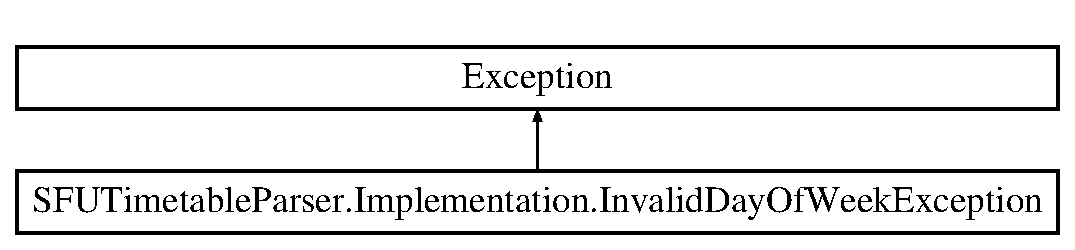
\includegraphics[height=2.000000cm]{class_s_f_u_timetable_parser_1_1_implementation_1_1_invalid_day_of_week_exception}
\end{center}
\end{figure}


Объявления и описания членов класса находятся в файле\+:\begin{DoxyCompactItemize}
\item 
S\+F\+U\+Timetable\+Parser.\+Implementation/\hyperlink{_invalid_day_of_week_exception_8cs}{Invalid\+Day\+Of\+Week\+Exception.\+cs}\end{DoxyCompactItemize}

\hypertarget{class_s_f_u_timetable_parser_1_1_core_1_1_exceptions_1_1_invalid_group_name_exception}{}\section{Класс S\+F\+U\+Timetable\+Parser.\+Core.\+Exceptions.\+Invalid\+Group\+Name\+Exception}
\label{class_s_f_u_timetable_parser_1_1_core_1_1_exceptions_1_1_invalid_group_name_exception}\index{S\+F\+U\+Timetable\+Parser.\+Core.\+Exceptions.\+Invalid\+Group\+Name\+Exception@{S\+F\+U\+Timetable\+Parser.\+Core.\+Exceptions.\+Invalid\+Group\+Name\+Exception}}
Граф наследования\+:S\+F\+U\+Timetable\+Parser.\+Core.\+Exceptions.\+Invalid\+Group\+Name\+Exception\+:\begin{figure}[H]
\begin{center}
\leavevmode
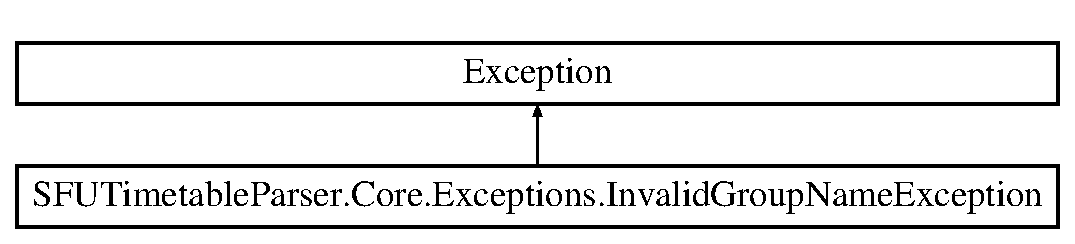
\includegraphics[height=2.000000cm]{class_s_f_u_timetable_parser_1_1_core_1_1_exceptions_1_1_invalid_group_name_exception}
\end{center}
\end{figure}
\subsection*{Открытые члены}
\begin{DoxyCompactItemize}
\item 
\hyperlink{class_s_f_u_timetable_parser_1_1_core_1_1_exceptions_1_1_invalid_group_name_exception_ac515d9024afadd1552e8856271624a29}{Invalid\+Group\+Name\+Exception} (string group\+Name)
\item 
\hyperlink{class_s_f_u_timetable_parser_1_1_core_1_1_exceptions_1_1_invalid_group_name_exception_a73275a887b6824dc48d7b2b17e0c8331}{Invalid\+Group\+Name\+Exception} (string group\+Name, string message)
\end{DoxyCompactItemize}
\subsection*{Свойства}
\begin{DoxyCompactItemize}
\item 
string \hyperlink{class_s_f_u_timetable_parser_1_1_core_1_1_exceptions_1_1_invalid_group_name_exception_a721ab32f677d9928aa65eb266427ab5b}{Group\+Name}\hspace{0.3cm}{\ttfamily  \mbox{[}get, set\mbox{]}}
\end{DoxyCompactItemize}


\subsection{Конструктор(ы)}
\mbox{\Hypertarget{class_s_f_u_timetable_parser_1_1_core_1_1_exceptions_1_1_invalid_group_name_exception_ac515d9024afadd1552e8856271624a29}\label{class_s_f_u_timetable_parser_1_1_core_1_1_exceptions_1_1_invalid_group_name_exception_ac515d9024afadd1552e8856271624a29}} 
\index{S\+F\+U\+Timetable\+Parser\+::\+Core\+::\+Exceptions\+::\+Invalid\+Group\+Name\+Exception@{S\+F\+U\+Timetable\+Parser\+::\+Core\+::\+Exceptions\+::\+Invalid\+Group\+Name\+Exception}!Invalid\+Group\+Name\+Exception@{Invalid\+Group\+Name\+Exception}}
\index{Invalid\+Group\+Name\+Exception@{Invalid\+Group\+Name\+Exception}!S\+F\+U\+Timetable\+Parser\+::\+Core\+::\+Exceptions\+::\+Invalid\+Group\+Name\+Exception@{S\+F\+U\+Timetable\+Parser\+::\+Core\+::\+Exceptions\+::\+Invalid\+Group\+Name\+Exception}}
\subsubsection{\texorpdfstring{Invalid\+Group\+Name\+Exception()}{InvalidGroupNameException()}\hspace{0.1cm}{\footnotesize\ttfamily [1/2]}}
{\footnotesize\ttfamily S\+F\+U\+Timetable\+Parser.\+Core.\+Exceptions.\+Invalid\+Group\+Name\+Exception.\+Invalid\+Group\+Name\+Exception (\begin{DoxyParamCaption}\item[{string}]{group\+Name }\end{DoxyParamCaption})}

\mbox{\Hypertarget{class_s_f_u_timetable_parser_1_1_core_1_1_exceptions_1_1_invalid_group_name_exception_a73275a887b6824dc48d7b2b17e0c8331}\label{class_s_f_u_timetable_parser_1_1_core_1_1_exceptions_1_1_invalid_group_name_exception_a73275a887b6824dc48d7b2b17e0c8331}} 
\index{S\+F\+U\+Timetable\+Parser\+::\+Core\+::\+Exceptions\+::\+Invalid\+Group\+Name\+Exception@{S\+F\+U\+Timetable\+Parser\+::\+Core\+::\+Exceptions\+::\+Invalid\+Group\+Name\+Exception}!Invalid\+Group\+Name\+Exception@{Invalid\+Group\+Name\+Exception}}
\index{Invalid\+Group\+Name\+Exception@{Invalid\+Group\+Name\+Exception}!S\+F\+U\+Timetable\+Parser\+::\+Core\+::\+Exceptions\+::\+Invalid\+Group\+Name\+Exception@{S\+F\+U\+Timetable\+Parser\+::\+Core\+::\+Exceptions\+::\+Invalid\+Group\+Name\+Exception}}
\subsubsection{\texorpdfstring{Invalid\+Group\+Name\+Exception()}{InvalidGroupNameException()}\hspace{0.1cm}{\footnotesize\ttfamily [2/2]}}
{\footnotesize\ttfamily S\+F\+U\+Timetable\+Parser.\+Core.\+Exceptions.\+Invalid\+Group\+Name\+Exception.\+Invalid\+Group\+Name\+Exception (\begin{DoxyParamCaption}\item[{string}]{group\+Name,  }\item[{string}]{message }\end{DoxyParamCaption})}



\subsection{Полный список свойств}
\mbox{\Hypertarget{class_s_f_u_timetable_parser_1_1_core_1_1_exceptions_1_1_invalid_group_name_exception_a721ab32f677d9928aa65eb266427ab5b}\label{class_s_f_u_timetable_parser_1_1_core_1_1_exceptions_1_1_invalid_group_name_exception_a721ab32f677d9928aa65eb266427ab5b}} 
\index{S\+F\+U\+Timetable\+Parser\+::\+Core\+::\+Exceptions\+::\+Invalid\+Group\+Name\+Exception@{S\+F\+U\+Timetable\+Parser\+::\+Core\+::\+Exceptions\+::\+Invalid\+Group\+Name\+Exception}!Group\+Name@{Group\+Name}}
\index{Group\+Name@{Group\+Name}!S\+F\+U\+Timetable\+Parser\+::\+Core\+::\+Exceptions\+::\+Invalid\+Group\+Name\+Exception@{S\+F\+U\+Timetable\+Parser\+::\+Core\+::\+Exceptions\+::\+Invalid\+Group\+Name\+Exception}}
\subsubsection{\texorpdfstring{Group\+Name}{GroupName}}
{\footnotesize\ttfamily string S\+F\+U\+Timetable\+Parser.\+Core.\+Exceptions.\+Invalid\+Group\+Name\+Exception.\+Group\+Name\hspace{0.3cm}{\ttfamily [get]}, {\ttfamily [set]}}



Объявления и описания членов класса находятся в файле\+:\begin{DoxyCompactItemize}
\item 
S\+F\+U\+Timetable\+Parser.\+Core/\+Exceptions/\hyperlink{_invalid_group_name_exception_8cs}{Invalid\+Group\+Name\+Exception.\+cs}\end{DoxyCompactItemize}

\hypertarget{interface_s_f_u_timetable_parser_1_1_core_1_1_i_timetable_manager}{}\section{Интерфейс S\+F\+U\+Timetable\+Parser.\+Core.\+I\+Timetable\+Manager}
\label{interface_s_f_u_timetable_parser_1_1_core_1_1_i_timetable_manager}\index{S\+F\+U\+Timetable\+Parser.\+Core.\+I\+Timetable\+Manager@{S\+F\+U\+Timetable\+Parser.\+Core.\+I\+Timetable\+Manager}}
Граф наследования\+:S\+F\+U\+Timetable\+Parser.\+Core.\+I\+Timetable\+Manager\+:\begin{figure}[H]
\begin{center}
\leavevmode
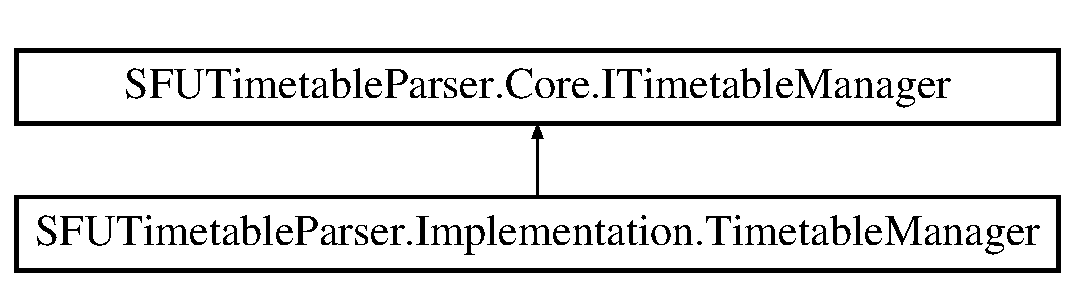
\includegraphics[height=2.000000cm]{interface_s_f_u_timetable_parser_1_1_core_1_1_i_timetable_manager}
\end{center}
\end{figure}
\subsection*{Открытые члены}
\begin{DoxyCompactItemize}
\item 
\hyperlink{class_s_f_u_timetable_parser_1_1_core_1_1_entities_1_1_group_timetable}{Group\+Timetable} \hyperlink{interface_s_f_u_timetable_parser_1_1_core_1_1_i_timetable_manager_aeb182ac554490f3c0db80691c1a8f739}{Get\+Group\+Timetable} (string group\+Name)
\begin{DoxyCompactList}\small\item\em Возвращает расписание заданной группы \end{DoxyCompactList}\item 
Task \hyperlink{interface_s_f_u_timetable_parser_1_1_core_1_1_i_timetable_manager_a4bc85e98ca57c83c9fa433036f064016}{Load\+Data\+Async} ()
\end{DoxyCompactItemize}
\subsection*{Свойства}
\begin{DoxyCompactItemize}
\item 
I\+Enumerable$<$ \hyperlink{class_s_f_u_timetable_parser_1_1_core_1_1_entities_1_1_group_timetable}{Group\+Timetable} $>$ \hyperlink{interface_s_f_u_timetable_parser_1_1_core_1_1_i_timetable_manager_ac092d73b1bfbbc5b5f1f50cb2234d622}{Timetable}\hspace{0.3cm}{\ttfamily  \mbox{[}get\mbox{]}}
\item 
I\+Enumerable$<$ string $>$ \hyperlink{interface_s_f_u_timetable_parser_1_1_core_1_1_i_timetable_manager_a9902fba6fdbe6a7050bd0ec81c6f0639}{Institutes}\hspace{0.3cm}{\ttfamily  \mbox{[}get\mbox{]}}
\item 
I\+Enumerable$<$ string $>$ \hyperlink{interface_s_f_u_timetable_parser_1_1_core_1_1_i_timetable_manager_aa783c9659f88b59d3d5e97a91eb0764c}{Subjects}\hspace{0.3cm}{\ttfamily  \mbox{[}get\mbox{]}}
\item 
I\+Enumerable$<$ string $>$ \hyperlink{interface_s_f_u_timetable_parser_1_1_core_1_1_i_timetable_manager_af5f2f109ae2194ec9737a0d5242579f0}{Groups}\hspace{0.3cm}{\ttfamily  \mbox{[}get\mbox{]}}
\end{DoxyCompactItemize}


\subsection{Подробное описание}
Основной интерфейс, содержащий методы и свойства для работы с расписанием 

\subsection{Методы}
\mbox{\Hypertarget{interface_s_f_u_timetable_parser_1_1_core_1_1_i_timetable_manager_aeb182ac554490f3c0db80691c1a8f739}\label{interface_s_f_u_timetable_parser_1_1_core_1_1_i_timetable_manager_aeb182ac554490f3c0db80691c1a8f739}} 
\index{S\+F\+U\+Timetable\+Parser\+::\+Core\+::\+I\+Timetable\+Manager@{S\+F\+U\+Timetable\+Parser\+::\+Core\+::\+I\+Timetable\+Manager}!Get\+Group\+Timetable@{Get\+Group\+Timetable}}
\index{Get\+Group\+Timetable@{Get\+Group\+Timetable}!S\+F\+U\+Timetable\+Parser\+::\+Core\+::\+I\+Timetable\+Manager@{S\+F\+U\+Timetable\+Parser\+::\+Core\+::\+I\+Timetable\+Manager}}
\subsubsection{\texorpdfstring{Get\+Group\+Timetable()}{GetGroupTimetable()}}
{\footnotesize\ttfamily \hyperlink{class_s_f_u_timetable_parser_1_1_core_1_1_entities_1_1_group_timetable}{Group\+Timetable} S\+F\+U\+Timetable\+Parser.\+Core.\+I\+Timetable\+Manager.\+Get\+Group\+Timetable (\begin{DoxyParamCaption}\item[{string}]{group\+Name }\end{DoxyParamCaption})}



Возвращает расписание заданной группы 


\begin{DoxyParams}{Аргументы}
{\em Название} & группы \\
\hline
\end{DoxyParams}


Замещается в \hyperlink{class_s_f_u_timetable_parser_1_1_implementation_1_1_timetable_manager_a23e17cd28ece08c67288e569380c9602}{S\+F\+U\+Timetable\+Parser.\+Implementation.\+Timetable\+Manager}.

\mbox{\Hypertarget{interface_s_f_u_timetable_parser_1_1_core_1_1_i_timetable_manager_a4bc85e98ca57c83c9fa433036f064016}\label{interface_s_f_u_timetable_parser_1_1_core_1_1_i_timetable_manager_a4bc85e98ca57c83c9fa433036f064016}} 
\index{S\+F\+U\+Timetable\+Parser\+::\+Core\+::\+I\+Timetable\+Manager@{S\+F\+U\+Timetable\+Parser\+::\+Core\+::\+I\+Timetable\+Manager}!Load\+Data\+Async@{Load\+Data\+Async}}
\index{Load\+Data\+Async@{Load\+Data\+Async}!S\+F\+U\+Timetable\+Parser\+::\+Core\+::\+I\+Timetable\+Manager@{S\+F\+U\+Timetable\+Parser\+::\+Core\+::\+I\+Timetable\+Manager}}
\subsubsection{\texorpdfstring{Load\+Data\+Async()}{LoadDataAsync()}}
{\footnotesize\ttfamily Task S\+F\+U\+Timetable\+Parser.\+Core.\+I\+Timetable\+Manager.\+Load\+Data\+Async (\begin{DoxyParamCaption}{ }\end{DoxyParamCaption})}

Асинхронный метод, используемы для загрузки данных с сафта СФУ 

Замещается в \hyperlink{class_s_f_u_timetable_parser_1_1_implementation_1_1_timetable_manager_a68266c332dfb29c133aaa36afd29385f}{S\+F\+U\+Timetable\+Parser.\+Implementation.\+Timetable\+Manager}.



\subsection{Полный список свойств}
\mbox{\Hypertarget{interface_s_f_u_timetable_parser_1_1_core_1_1_i_timetable_manager_af5f2f109ae2194ec9737a0d5242579f0}\label{interface_s_f_u_timetable_parser_1_1_core_1_1_i_timetable_manager_af5f2f109ae2194ec9737a0d5242579f0}} 
\index{S\+F\+U\+Timetable\+Parser\+::\+Core\+::\+I\+Timetable\+Manager@{S\+F\+U\+Timetable\+Parser\+::\+Core\+::\+I\+Timetable\+Manager}!Groups@{Groups}}
\index{Groups@{Groups}!S\+F\+U\+Timetable\+Parser\+::\+Core\+::\+I\+Timetable\+Manager@{S\+F\+U\+Timetable\+Parser\+::\+Core\+::\+I\+Timetable\+Manager}}
\subsubsection{\texorpdfstring{Groups}{Groups}}
{\footnotesize\ttfamily I\+Enumerable$<$string$>$ S\+F\+U\+Timetable\+Parser.\+Core.\+I\+Timetable\+Manager.\+Groups\hspace{0.3cm}{\ttfamily [get]}}

Свойство, возвращающее список групп \mbox{\Hypertarget{interface_s_f_u_timetable_parser_1_1_core_1_1_i_timetable_manager_a9902fba6fdbe6a7050bd0ec81c6f0639}\label{interface_s_f_u_timetable_parser_1_1_core_1_1_i_timetable_manager_a9902fba6fdbe6a7050bd0ec81c6f0639}} 
\index{S\+F\+U\+Timetable\+Parser\+::\+Core\+::\+I\+Timetable\+Manager@{S\+F\+U\+Timetable\+Parser\+::\+Core\+::\+I\+Timetable\+Manager}!Institutes@{Institutes}}
\index{Institutes@{Institutes}!S\+F\+U\+Timetable\+Parser\+::\+Core\+::\+I\+Timetable\+Manager@{S\+F\+U\+Timetable\+Parser\+::\+Core\+::\+I\+Timetable\+Manager}}
\subsubsection{\texorpdfstring{Institutes}{Institutes}}
{\footnotesize\ttfamily I\+Enumerable$<$string$>$ S\+F\+U\+Timetable\+Parser.\+Core.\+I\+Timetable\+Manager.\+Institutes\hspace{0.3cm}{\ttfamily [get]}}

Свойство, возвращающее список институтов \mbox{\Hypertarget{interface_s_f_u_timetable_parser_1_1_core_1_1_i_timetable_manager_aa783c9659f88b59d3d5e97a91eb0764c}\label{interface_s_f_u_timetable_parser_1_1_core_1_1_i_timetable_manager_aa783c9659f88b59d3d5e97a91eb0764c}} 
\index{S\+F\+U\+Timetable\+Parser\+::\+Core\+::\+I\+Timetable\+Manager@{S\+F\+U\+Timetable\+Parser\+::\+Core\+::\+I\+Timetable\+Manager}!Subjects@{Subjects}}
\index{Subjects@{Subjects}!S\+F\+U\+Timetable\+Parser\+::\+Core\+::\+I\+Timetable\+Manager@{S\+F\+U\+Timetable\+Parser\+::\+Core\+::\+I\+Timetable\+Manager}}
\subsubsection{\texorpdfstring{Subjects}{Subjects}}
{\footnotesize\ttfamily I\+Enumerable$<$string$>$ S\+F\+U\+Timetable\+Parser.\+Core.\+I\+Timetable\+Manager.\+Subjects\hspace{0.3cm}{\ttfamily [get]}}

Свойство, возвращающее список предметов \mbox{\Hypertarget{interface_s_f_u_timetable_parser_1_1_core_1_1_i_timetable_manager_ac092d73b1bfbbc5b5f1f50cb2234d622}\label{interface_s_f_u_timetable_parser_1_1_core_1_1_i_timetable_manager_ac092d73b1bfbbc5b5f1f50cb2234d622}} 
\index{S\+F\+U\+Timetable\+Parser\+::\+Core\+::\+I\+Timetable\+Manager@{S\+F\+U\+Timetable\+Parser\+::\+Core\+::\+I\+Timetable\+Manager}!Timetable@{Timetable}}
\index{Timetable@{Timetable}!S\+F\+U\+Timetable\+Parser\+::\+Core\+::\+I\+Timetable\+Manager@{S\+F\+U\+Timetable\+Parser\+::\+Core\+::\+I\+Timetable\+Manager}}
\subsubsection{\texorpdfstring{Timetable}{Timetable}}
{\footnotesize\ttfamily I\+Enumerable$<$\hyperlink{class_s_f_u_timetable_parser_1_1_core_1_1_entities_1_1_group_timetable}{Group\+Timetable}$>$ S\+F\+U\+Timetable\+Parser.\+Core.\+I\+Timetable\+Manager.\+Timetable\hspace{0.3cm}{\ttfamily [get]}}

Свойство, возвращающее список моделей распиания всех групп 

Объявления и описания членов интерфейса находятся в файле\+:\begin{DoxyCompactItemize}
\item 
S\+F\+U\+Timetable\+Parser.\+Core/\hyperlink{_i_timetable_manager_8cs}{I\+Timetable\+Manager.\+cs}\end{DoxyCompactItemize}

\hypertarget{class_s_f_u_timetable_parser_1_1_core_1_1_entities_1_1_professor}{}\section{Класс S\+F\+U\+Timetable\+Parser.\+Core.\+Entities.\+Professor}
\label{class_s_f_u_timetable_parser_1_1_core_1_1_entities_1_1_professor}\index{S\+F\+U\+Timetable\+Parser.\+Core.\+Entities.\+Professor@{S\+F\+U\+Timetable\+Parser.\+Core.\+Entities.\+Professor}}
\subsection*{Свойства}
\begin{DoxyCompactItemize}
\item 
string \hyperlink{class_s_f_u_timetable_parser_1_1_core_1_1_entities_1_1_professor_aef0a660b8ec7c3fe098fd05f1c150849}{Name}\hspace{0.3cm}{\ttfamily  \mbox{[}get, set\mbox{]}}
\item 
string \hyperlink{class_s_f_u_timetable_parser_1_1_core_1_1_entities_1_1_professor_af12c8b78e929132a07b6ecbb47459978}{Surname}\hspace{0.3cm}{\ttfamily  \mbox{[}get, set\mbox{]}}
\item 
string \hyperlink{class_s_f_u_timetable_parser_1_1_core_1_1_entities_1_1_professor_a0b10ef5eb622879e43685d3b0794fb18}{Patronymic}\hspace{0.3cm}{\ttfamily  \mbox{[}get, set\mbox{]}}
\end{DoxyCompactItemize}


\subsection{Подробное описание}
Моедль преподавателя 

\subsection{Полный список свойств}
\mbox{\Hypertarget{class_s_f_u_timetable_parser_1_1_core_1_1_entities_1_1_professor_aef0a660b8ec7c3fe098fd05f1c150849}\label{class_s_f_u_timetable_parser_1_1_core_1_1_entities_1_1_professor_aef0a660b8ec7c3fe098fd05f1c150849}} 
\index{S\+F\+U\+Timetable\+Parser\+::\+Core\+::\+Entities\+::\+Professor@{S\+F\+U\+Timetable\+Parser\+::\+Core\+::\+Entities\+::\+Professor}!Name@{Name}}
\index{Name@{Name}!S\+F\+U\+Timetable\+Parser\+::\+Core\+::\+Entities\+::\+Professor@{S\+F\+U\+Timetable\+Parser\+::\+Core\+::\+Entities\+::\+Professor}}
\subsubsection{\texorpdfstring{Name}{Name}}
{\footnotesize\ttfamily string S\+F\+U\+Timetable\+Parser.\+Core.\+Entities.\+Professor.\+Name\hspace{0.3cm}{\ttfamily [get]}, {\ttfamily [set]}}

\mbox{\Hypertarget{class_s_f_u_timetable_parser_1_1_core_1_1_entities_1_1_professor_a0b10ef5eb622879e43685d3b0794fb18}\label{class_s_f_u_timetable_parser_1_1_core_1_1_entities_1_1_professor_a0b10ef5eb622879e43685d3b0794fb18}} 
\index{S\+F\+U\+Timetable\+Parser\+::\+Core\+::\+Entities\+::\+Professor@{S\+F\+U\+Timetable\+Parser\+::\+Core\+::\+Entities\+::\+Professor}!Patronymic@{Patronymic}}
\index{Patronymic@{Patronymic}!S\+F\+U\+Timetable\+Parser\+::\+Core\+::\+Entities\+::\+Professor@{S\+F\+U\+Timetable\+Parser\+::\+Core\+::\+Entities\+::\+Professor}}
\subsubsection{\texorpdfstring{Patronymic}{Patronymic}}
{\footnotesize\ttfamily string S\+F\+U\+Timetable\+Parser.\+Core.\+Entities.\+Professor.\+Patronymic\hspace{0.3cm}{\ttfamily [get]}, {\ttfamily [set]}}

\mbox{\Hypertarget{class_s_f_u_timetable_parser_1_1_core_1_1_entities_1_1_professor_af12c8b78e929132a07b6ecbb47459978}\label{class_s_f_u_timetable_parser_1_1_core_1_1_entities_1_1_professor_af12c8b78e929132a07b6ecbb47459978}} 
\index{S\+F\+U\+Timetable\+Parser\+::\+Core\+::\+Entities\+::\+Professor@{S\+F\+U\+Timetable\+Parser\+::\+Core\+::\+Entities\+::\+Professor}!Surname@{Surname}}
\index{Surname@{Surname}!S\+F\+U\+Timetable\+Parser\+::\+Core\+::\+Entities\+::\+Professor@{S\+F\+U\+Timetable\+Parser\+::\+Core\+::\+Entities\+::\+Professor}}
\subsubsection{\texorpdfstring{Surname}{Surname}}
{\footnotesize\ttfamily string S\+F\+U\+Timetable\+Parser.\+Core.\+Entities.\+Professor.\+Surname\hspace{0.3cm}{\ttfamily [get]}, {\ttfamily [set]}}



Объявления и описания членов класса находятся в файле\+:\begin{DoxyCompactItemize}
\item 
S\+F\+U\+Timetable\+Parser.\+Core/\+Entities/\hyperlink{_professor_8cs}{Professor.\+cs}\end{DoxyCompactItemize}

\hypertarget{class_s_f_u_timetable_parser_1_1_core_1_1_entities_1_1_subject_model}{}\section{Класс S\+F\+U\+Timetable\+Parser.\+Core.\+Entities.\+Subject\+Model}
\label{class_s_f_u_timetable_parser_1_1_core_1_1_entities_1_1_subject_model}\index{S\+F\+U\+Timetable\+Parser.\+Core.\+Entities.\+Subject\+Model@{S\+F\+U\+Timetable\+Parser.\+Core.\+Entities.\+Subject\+Model}}
\subsection*{Свойства}
\begin{DoxyCompactItemize}
\item 
string \hyperlink{class_s_f_u_timetable_parser_1_1_core_1_1_entities_1_1_subject_model_aa9ff8815894d5afab78f96d88e4af542}{Name}\hspace{0.3cm}{\ttfamily  \mbox{[}get, set\mbox{]}}
\begin{DoxyCompactList}\small\item\em Название \end{DoxyCompactList}\item 
string \hyperlink{class_s_f_u_timetable_parser_1_1_core_1_1_entities_1_1_subject_model_a7852f100383c1d51c859d5386944401a}{Type}\hspace{0.3cm}{\ttfamily  \mbox{[}get, set\mbox{]}}
\begin{DoxyCompactList}\small\item\em Тип (лекция или практика) \end{DoxyCompactList}\item 
string \hyperlink{class_s_f_u_timetable_parser_1_1_core_1_1_entities_1_1_subject_model_ae36a75954dccfdc388ef3cbdfc1a05ac}{Auditory}\hspace{0.3cm}{\ttfamily  \mbox{[}get, set\mbox{]}}
\begin{DoxyCompactList}\small\item\em Аудитория \end{DoxyCompactList}\item 
\hyperlink{class_s_f_u_timetable_parser_1_1_core_1_1_entities_1_1_professor}{Professor} \hyperlink{class_s_f_u_timetable_parser_1_1_core_1_1_entities_1_1_subject_model_ac0d805823baea8d8b5330ca0ab70593b}{Professor}\hspace{0.3cm}{\ttfamily  \mbox{[}get, set\mbox{]}}
\begin{DoxyCompactList}\small\item\em Модель преподавателя \end{DoxyCompactList}\end{DoxyCompactItemize}


\subsection{Подробное описание}
Модель предмета в расписании 

\subsection{Полный список свойств}
\mbox{\Hypertarget{class_s_f_u_timetable_parser_1_1_core_1_1_entities_1_1_subject_model_ae36a75954dccfdc388ef3cbdfc1a05ac}\label{class_s_f_u_timetable_parser_1_1_core_1_1_entities_1_1_subject_model_ae36a75954dccfdc388ef3cbdfc1a05ac}} 
\index{S\+F\+U\+Timetable\+Parser\+::\+Core\+::\+Entities\+::\+Subject\+Model@{S\+F\+U\+Timetable\+Parser\+::\+Core\+::\+Entities\+::\+Subject\+Model}!Auditory@{Auditory}}
\index{Auditory@{Auditory}!S\+F\+U\+Timetable\+Parser\+::\+Core\+::\+Entities\+::\+Subject\+Model@{S\+F\+U\+Timetable\+Parser\+::\+Core\+::\+Entities\+::\+Subject\+Model}}
\subsubsection{\texorpdfstring{Auditory}{Auditory}}
{\footnotesize\ttfamily string S\+F\+U\+Timetable\+Parser.\+Core.\+Entities.\+Subject\+Model.\+Auditory\hspace{0.3cm}{\ttfamily [get]}, {\ttfamily [set]}}



Аудитория 

\mbox{\Hypertarget{class_s_f_u_timetable_parser_1_1_core_1_1_entities_1_1_subject_model_aa9ff8815894d5afab78f96d88e4af542}\label{class_s_f_u_timetable_parser_1_1_core_1_1_entities_1_1_subject_model_aa9ff8815894d5afab78f96d88e4af542}} 
\index{S\+F\+U\+Timetable\+Parser\+::\+Core\+::\+Entities\+::\+Subject\+Model@{S\+F\+U\+Timetable\+Parser\+::\+Core\+::\+Entities\+::\+Subject\+Model}!Name@{Name}}
\index{Name@{Name}!S\+F\+U\+Timetable\+Parser\+::\+Core\+::\+Entities\+::\+Subject\+Model@{S\+F\+U\+Timetable\+Parser\+::\+Core\+::\+Entities\+::\+Subject\+Model}}
\subsubsection{\texorpdfstring{Name}{Name}}
{\footnotesize\ttfamily string S\+F\+U\+Timetable\+Parser.\+Core.\+Entities.\+Subject\+Model.\+Name\hspace{0.3cm}{\ttfamily [get]}, {\ttfamily [set]}}



Название 

\mbox{\Hypertarget{class_s_f_u_timetable_parser_1_1_core_1_1_entities_1_1_subject_model_ac0d805823baea8d8b5330ca0ab70593b}\label{class_s_f_u_timetable_parser_1_1_core_1_1_entities_1_1_subject_model_ac0d805823baea8d8b5330ca0ab70593b}} 
\index{S\+F\+U\+Timetable\+Parser\+::\+Core\+::\+Entities\+::\+Subject\+Model@{S\+F\+U\+Timetable\+Parser\+::\+Core\+::\+Entities\+::\+Subject\+Model}!Professor@{Professor}}
\index{Professor@{Professor}!S\+F\+U\+Timetable\+Parser\+::\+Core\+::\+Entities\+::\+Subject\+Model@{S\+F\+U\+Timetable\+Parser\+::\+Core\+::\+Entities\+::\+Subject\+Model}}
\subsubsection{\texorpdfstring{Professor}{Professor}}
{\footnotesize\ttfamily \hyperlink{class_s_f_u_timetable_parser_1_1_core_1_1_entities_1_1_professor}{Professor} S\+F\+U\+Timetable\+Parser.\+Core.\+Entities.\+Subject\+Model.\+Professor\hspace{0.3cm}{\ttfamily [get]}, {\ttfamily [set]}}



Модель преподавателя 

\mbox{\Hypertarget{class_s_f_u_timetable_parser_1_1_core_1_1_entities_1_1_subject_model_a7852f100383c1d51c859d5386944401a}\label{class_s_f_u_timetable_parser_1_1_core_1_1_entities_1_1_subject_model_a7852f100383c1d51c859d5386944401a}} 
\index{S\+F\+U\+Timetable\+Parser\+::\+Core\+::\+Entities\+::\+Subject\+Model@{S\+F\+U\+Timetable\+Parser\+::\+Core\+::\+Entities\+::\+Subject\+Model}!Type@{Type}}
\index{Type@{Type}!S\+F\+U\+Timetable\+Parser\+::\+Core\+::\+Entities\+::\+Subject\+Model@{S\+F\+U\+Timetable\+Parser\+::\+Core\+::\+Entities\+::\+Subject\+Model}}
\subsubsection{\texorpdfstring{Type}{Type}}
{\footnotesize\ttfamily string S\+F\+U\+Timetable\+Parser.\+Core.\+Entities.\+Subject\+Model.\+Type\hspace{0.3cm}{\ttfamily [get]}, {\ttfamily [set]}}



Тип (лекция или практика) 



Объявления и описания членов класса находятся в файле\+:\begin{DoxyCompactItemize}
\item 
S\+F\+U\+Timetable\+Parser.\+Core/\+Entities/\hyperlink{_subject_model_8cs}{Subject\+Model.\+cs}\end{DoxyCompactItemize}

\hypertarget{class_s_f_u_timetable_parser_1_1_implementation_1_1_timetable_manager}{}\section{Класс S\+F\+U\+Timetable\+Parser.\+Implementation.\+Timetable\+Manager}
\label{class_s_f_u_timetable_parser_1_1_implementation_1_1_timetable_manager}\index{S\+F\+U\+Timetable\+Parser.\+Implementation.\+Timetable\+Manager@{S\+F\+U\+Timetable\+Parser.\+Implementation.\+Timetable\+Manager}}
Граф наследования\+:S\+F\+U\+Timetable\+Parser.\+Implementation.\+Timetable\+Manager\+:\begin{figure}[H]
\begin{center}
\leavevmode
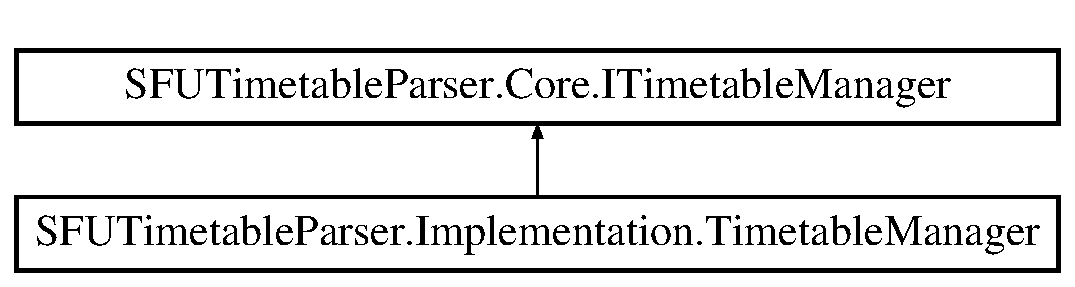
\includegraphics[height=2.000000cm]{class_s_f_u_timetable_parser_1_1_implementation_1_1_timetable_manager}
\end{center}
\end{figure}
\subsection*{Открытые члены}
\begin{DoxyCompactItemize}
\item 
\hyperlink{class_s_f_u_timetable_parser_1_1_implementation_1_1_timetable_manager_adc6225553917e6907461c1e127084dcb}{Timetable\+Manager} ()
\item 
\hyperlink{class_s_f_u_timetable_parser_1_1_core_1_1_entities_1_1_group_timetable}{Group\+Timetable} \hyperlink{class_s_f_u_timetable_parser_1_1_implementation_1_1_timetable_manager_a23e17cd28ece08c67288e569380c9602}{Get\+Group\+Timetable} (string group\+Name)
\begin{DoxyCompactList}\small\item\em Возвращает расписание заданной группы \end{DoxyCompactList}\item 
async Task \hyperlink{class_s_f_u_timetable_parser_1_1_implementation_1_1_timetable_manager_a68266c332dfb29c133aaa36afd29385f}{Load\+Data\+Async} ()
\end{DoxyCompactItemize}
\subsection*{Свойства}
\begin{DoxyCompactItemize}
\item 
I\+Enumerable$<$ \hyperlink{class_s_f_u_timetable_parser_1_1_core_1_1_entities_1_1_group_timetable}{Group\+Timetable} $>$ \hyperlink{class_s_f_u_timetable_parser_1_1_implementation_1_1_timetable_manager_a147d539c841ac942201c132013d0293f}{Timetable}\hspace{0.3cm}{\ttfamily  \mbox{[}get\mbox{]}}
\item 
I\+Enumerable$<$ string $>$ \hyperlink{class_s_f_u_timetable_parser_1_1_implementation_1_1_timetable_manager_a7b8c8acd9e266e41f023ac57b6f88209}{Subjects}\hspace{0.3cm}{\ttfamily  \mbox{[}get\mbox{]}}
\item 
I\+Enumerable$<$ string $>$ \hyperlink{class_s_f_u_timetable_parser_1_1_implementation_1_1_timetable_manager_a382d2dd82077238efd4dbc224e3ac44a}{Groups}\hspace{0.3cm}{\ttfamily  \mbox{[}get\mbox{]}}
\item 
I\+Enumerable$<$ string $>$ \hyperlink{class_s_f_u_timetable_parser_1_1_implementation_1_1_timetable_manager_a15bc77e455cc8e9add14f7131887aa8e}{Institutes}\hspace{0.3cm}{\ttfamily  \mbox{[}get\mbox{]}}
\end{DoxyCompactItemize}


\subsection{Подробное описание}
Реализация основного интерфейса для работы с раписанием 

\subsection{Конструктор(ы)}
\mbox{\Hypertarget{class_s_f_u_timetable_parser_1_1_implementation_1_1_timetable_manager_adc6225553917e6907461c1e127084dcb}\label{class_s_f_u_timetable_parser_1_1_implementation_1_1_timetable_manager_adc6225553917e6907461c1e127084dcb}} 
\index{S\+F\+U\+Timetable\+Parser\+::\+Implementation\+::\+Timetable\+Manager@{S\+F\+U\+Timetable\+Parser\+::\+Implementation\+::\+Timetable\+Manager}!Timetable\+Manager@{Timetable\+Manager}}
\index{Timetable\+Manager@{Timetable\+Manager}!S\+F\+U\+Timetable\+Parser\+::\+Implementation\+::\+Timetable\+Manager@{S\+F\+U\+Timetable\+Parser\+::\+Implementation\+::\+Timetable\+Manager}}
\subsubsection{\texorpdfstring{Timetable\+Manager()}{TimetableManager()}}
{\footnotesize\ttfamily S\+F\+U\+Timetable\+Parser.\+Implementation.\+Timetable\+Manager.\+Timetable\+Manager (\begin{DoxyParamCaption}{ }\end{DoxyParamCaption})}

Стандартный конструктор 

\subsection{Методы}
\mbox{\Hypertarget{class_s_f_u_timetable_parser_1_1_implementation_1_1_timetable_manager_a23e17cd28ece08c67288e569380c9602}\label{class_s_f_u_timetable_parser_1_1_implementation_1_1_timetable_manager_a23e17cd28ece08c67288e569380c9602}} 
\index{S\+F\+U\+Timetable\+Parser\+::\+Implementation\+::\+Timetable\+Manager@{S\+F\+U\+Timetable\+Parser\+::\+Implementation\+::\+Timetable\+Manager}!Get\+Group\+Timetable@{Get\+Group\+Timetable}}
\index{Get\+Group\+Timetable@{Get\+Group\+Timetable}!S\+F\+U\+Timetable\+Parser\+::\+Implementation\+::\+Timetable\+Manager@{S\+F\+U\+Timetable\+Parser\+::\+Implementation\+::\+Timetable\+Manager}}
\subsubsection{\texorpdfstring{Get\+Group\+Timetable()}{GetGroupTimetable()}}
{\footnotesize\ttfamily \hyperlink{class_s_f_u_timetable_parser_1_1_core_1_1_entities_1_1_group_timetable}{Group\+Timetable} S\+F\+U\+Timetable\+Parser.\+Implementation.\+Timetable\+Manager.\+Get\+Group\+Timetable (\begin{DoxyParamCaption}\item[{string}]{group\+Name }\end{DoxyParamCaption})}



Возвращает расписание заданной группы 


\begin{DoxyParams}{Аргументы}
{\em Название} & группы \\
\hline
\end{DoxyParams}


Замещает \hyperlink{interface_s_f_u_timetable_parser_1_1_core_1_1_i_timetable_manager_aeb182ac554490f3c0db80691c1a8f739}{S\+F\+U\+Timetable\+Parser.\+Core.\+I\+Timetable\+Manager}.

\mbox{\Hypertarget{class_s_f_u_timetable_parser_1_1_implementation_1_1_timetable_manager_a68266c332dfb29c133aaa36afd29385f}\label{class_s_f_u_timetable_parser_1_1_implementation_1_1_timetable_manager_a68266c332dfb29c133aaa36afd29385f}} 
\index{S\+F\+U\+Timetable\+Parser\+::\+Implementation\+::\+Timetable\+Manager@{S\+F\+U\+Timetable\+Parser\+::\+Implementation\+::\+Timetable\+Manager}!Load\+Data\+Async@{Load\+Data\+Async}}
\index{Load\+Data\+Async@{Load\+Data\+Async}!S\+F\+U\+Timetable\+Parser\+::\+Implementation\+::\+Timetable\+Manager@{S\+F\+U\+Timetable\+Parser\+::\+Implementation\+::\+Timetable\+Manager}}
\subsubsection{\texorpdfstring{Load\+Data\+Async()}{LoadDataAsync()}}
{\footnotesize\ttfamily async Task S\+F\+U\+Timetable\+Parser.\+Implementation.\+Timetable\+Manager.\+Load\+Data\+Async (\begin{DoxyParamCaption}{ }\end{DoxyParamCaption})}

Асинхронный метод, используемы для загрузки данных с сафта СФУ 

Замещает \hyperlink{interface_s_f_u_timetable_parser_1_1_core_1_1_i_timetable_manager_a4bc85e98ca57c83c9fa433036f064016}{S\+F\+U\+Timetable\+Parser.\+Core.\+I\+Timetable\+Manager}.



\subsection{Полный список свойств}
\mbox{\Hypertarget{class_s_f_u_timetable_parser_1_1_implementation_1_1_timetable_manager_a382d2dd82077238efd4dbc224e3ac44a}\label{class_s_f_u_timetable_parser_1_1_implementation_1_1_timetable_manager_a382d2dd82077238efd4dbc224e3ac44a}} 
\index{S\+F\+U\+Timetable\+Parser\+::\+Implementation\+::\+Timetable\+Manager@{S\+F\+U\+Timetable\+Parser\+::\+Implementation\+::\+Timetable\+Manager}!Groups@{Groups}}
\index{Groups@{Groups}!S\+F\+U\+Timetable\+Parser\+::\+Implementation\+::\+Timetable\+Manager@{S\+F\+U\+Timetable\+Parser\+::\+Implementation\+::\+Timetable\+Manager}}
\subsubsection{\texorpdfstring{Groups}{Groups}}
{\footnotesize\ttfamily I\+Enumerable$<$string$>$ S\+F\+U\+Timetable\+Parser.\+Implementation.\+Timetable\+Manager.\+Groups\hspace{0.3cm}{\ttfamily [get]}}

Свойство, возвращающее список групп \mbox{\Hypertarget{class_s_f_u_timetable_parser_1_1_implementation_1_1_timetable_manager_a15bc77e455cc8e9add14f7131887aa8e}\label{class_s_f_u_timetable_parser_1_1_implementation_1_1_timetable_manager_a15bc77e455cc8e9add14f7131887aa8e}} 
\index{S\+F\+U\+Timetable\+Parser\+::\+Implementation\+::\+Timetable\+Manager@{S\+F\+U\+Timetable\+Parser\+::\+Implementation\+::\+Timetable\+Manager}!Institutes@{Institutes}}
\index{Institutes@{Institutes}!S\+F\+U\+Timetable\+Parser\+::\+Implementation\+::\+Timetable\+Manager@{S\+F\+U\+Timetable\+Parser\+::\+Implementation\+::\+Timetable\+Manager}}
\subsubsection{\texorpdfstring{Institutes}{Institutes}}
{\footnotesize\ttfamily I\+Enumerable$<$string$>$ S\+F\+U\+Timetable\+Parser.\+Implementation.\+Timetable\+Manager.\+Institutes\hspace{0.3cm}{\ttfamily [get]}}

Свойство, возвращающее список институтов \mbox{\Hypertarget{class_s_f_u_timetable_parser_1_1_implementation_1_1_timetable_manager_a7b8c8acd9e266e41f023ac57b6f88209}\label{class_s_f_u_timetable_parser_1_1_implementation_1_1_timetable_manager_a7b8c8acd9e266e41f023ac57b6f88209}} 
\index{S\+F\+U\+Timetable\+Parser\+::\+Implementation\+::\+Timetable\+Manager@{S\+F\+U\+Timetable\+Parser\+::\+Implementation\+::\+Timetable\+Manager}!Subjects@{Subjects}}
\index{Subjects@{Subjects}!S\+F\+U\+Timetable\+Parser\+::\+Implementation\+::\+Timetable\+Manager@{S\+F\+U\+Timetable\+Parser\+::\+Implementation\+::\+Timetable\+Manager}}
\subsubsection{\texorpdfstring{Subjects}{Subjects}}
{\footnotesize\ttfamily I\+Enumerable$<$string$>$ S\+F\+U\+Timetable\+Parser.\+Implementation.\+Timetable\+Manager.\+Subjects\hspace{0.3cm}{\ttfamily [get]}}

Свойство, возвращающее список предметов \mbox{\Hypertarget{class_s_f_u_timetable_parser_1_1_implementation_1_1_timetable_manager_a147d539c841ac942201c132013d0293f}\label{class_s_f_u_timetable_parser_1_1_implementation_1_1_timetable_manager_a147d539c841ac942201c132013d0293f}} 
\index{S\+F\+U\+Timetable\+Parser\+::\+Implementation\+::\+Timetable\+Manager@{S\+F\+U\+Timetable\+Parser\+::\+Implementation\+::\+Timetable\+Manager}!Timetable@{Timetable}}
\index{Timetable@{Timetable}!S\+F\+U\+Timetable\+Parser\+::\+Implementation\+::\+Timetable\+Manager@{S\+F\+U\+Timetable\+Parser\+::\+Implementation\+::\+Timetable\+Manager}}
\subsubsection{\texorpdfstring{Timetable}{Timetable}}
{\footnotesize\ttfamily I\+Enumerable$<$\hyperlink{class_s_f_u_timetable_parser_1_1_core_1_1_entities_1_1_group_timetable}{Group\+Timetable}$>$ S\+F\+U\+Timetable\+Parser.\+Implementation.\+Timetable\+Manager.\+Timetable\hspace{0.3cm}{\ttfamily [get]}}

Свойство, возвращающее список моделей распиания всех групп 

Объявления и описания членов класса находятся в файле\+:\begin{DoxyCompactItemize}
\item 
S\+F\+U\+Timetable\+Parser.\+Implementation/\hyperlink{_timetable_manager_8cs}{Timetable\+Manager.\+cs}\end{DoxyCompactItemize}

\hypertarget{class_s_f_u_timetable_parser_1_1_core_1_1_entities_1_1_timetable_record}{}\section{Класс S\+F\+U\+Timetable\+Parser.\+Core.\+Entities.\+Timetable\+Record}
\label{class_s_f_u_timetable_parser_1_1_core_1_1_entities_1_1_timetable_record}\index{S\+F\+U\+Timetable\+Parser.\+Core.\+Entities.\+Timetable\+Record@{S\+F\+U\+Timetable\+Parser.\+Core.\+Entities.\+Timetable\+Record}}
\subsection*{Открытые атрибуты}
\begin{DoxyCompactItemize}
\item 
bool \hyperlink{class_s_f_u_timetable_parser_1_1_core_1_1_entities_1_1_timetable_record_a9033a08965a70fced0f1644baf261563}{Depended\+On\+Week} =$>$ \hyperlink{class_s_f_u_timetable_parser_1_1_core_1_1_entities_1_1_timetable_record_a453625dea6c24ea69d5113ce9f60d994}{Subject\+On\+Even} != \hyperlink{class_s_f_u_timetable_parser_1_1_core_1_1_entities_1_1_timetable_record_a599e9b6010ce9af0447fa32c42948fb9}{Subject\+On\+Odd}
\begin{DoxyCompactList}\small\item\em Определяет, зависит ли предмет от номера недели \end{DoxyCompactList}\end{DoxyCompactItemize}
\subsection*{Свойства}
\begin{DoxyCompactItemize}
\item 
\hyperlink{class_s_f_u_timetable_parser_1_1_core_1_1_entities_1_1_subject_model}{Subject\+Model} \hyperlink{class_s_f_u_timetable_parser_1_1_core_1_1_entities_1_1_timetable_record_a453625dea6c24ea69d5113ce9f60d994}{Subject\+On\+Even}\hspace{0.3cm}{\ttfamily  \mbox{[}get, set\mbox{]}}
\begin{DoxyCompactList}\small\item\em Модель предмета по чётным неделям \end{DoxyCompactList}\item 
\hyperlink{class_s_f_u_timetable_parser_1_1_core_1_1_entities_1_1_subject_model}{Subject\+Model} \hyperlink{class_s_f_u_timetable_parser_1_1_core_1_1_entities_1_1_timetable_record_a599e9b6010ce9af0447fa32c42948fb9}{Subject\+On\+Odd}\hspace{0.3cm}{\ttfamily  \mbox{[}get, set\mbox{]}}
\begin{DoxyCompactList}\small\item\em Модель предмета по нечётным неделям \end{DoxyCompactList}\item 
string \hyperlink{class_s_f_u_timetable_parser_1_1_core_1_1_entities_1_1_timetable_record_aabd478fcff6c39b11dd7ec6a17379db0}{Period}\hspace{0.3cm}{\ttfamily  \mbox{[}get, set\mbox{]}}
\begin{DoxyCompactList}\small\item\em Строковое представление временного периода занятия \end{DoxyCompactList}\item 
int \hyperlink{class_s_f_u_timetable_parser_1_1_core_1_1_entities_1_1_timetable_record_a38e3cb5b0430d92d1a677abda0bf035d}{Number}\hspace{0.3cm}{\ttfamily  \mbox{[}get, set\mbox{]}}
\begin{DoxyCompactList}\small\item\em Порядковый номер занятия \end{DoxyCompactList}\end{DoxyCompactItemize}


\subsection{Подробное описание}
Запись дневного расписания 

\subsection{Данные класса}
\mbox{\Hypertarget{class_s_f_u_timetable_parser_1_1_core_1_1_entities_1_1_timetable_record_a9033a08965a70fced0f1644baf261563}\label{class_s_f_u_timetable_parser_1_1_core_1_1_entities_1_1_timetable_record_a9033a08965a70fced0f1644baf261563}} 
\index{S\+F\+U\+Timetable\+Parser\+::\+Core\+::\+Entities\+::\+Timetable\+Record@{S\+F\+U\+Timetable\+Parser\+::\+Core\+::\+Entities\+::\+Timetable\+Record}!Depended\+On\+Week@{Depended\+On\+Week}}
\index{Depended\+On\+Week@{Depended\+On\+Week}!S\+F\+U\+Timetable\+Parser\+::\+Core\+::\+Entities\+::\+Timetable\+Record@{S\+F\+U\+Timetable\+Parser\+::\+Core\+::\+Entities\+::\+Timetable\+Record}}
\subsubsection{\texorpdfstring{Depended\+On\+Week}{DependedOnWeek}}
{\footnotesize\ttfamily bool S\+F\+U\+Timetable\+Parser.\+Core.\+Entities.\+Timetable\+Record.\+Depended\+On\+Week =$>$ \hyperlink{class_s_f_u_timetable_parser_1_1_core_1_1_entities_1_1_timetable_record_a453625dea6c24ea69d5113ce9f60d994}{Subject\+On\+Even} != \hyperlink{class_s_f_u_timetable_parser_1_1_core_1_1_entities_1_1_timetable_record_a599e9b6010ce9af0447fa32c42948fb9}{Subject\+On\+Odd}}



Определяет, зависит ли предмет от номера недели 



\subsection{Полный список свойств}
\mbox{\Hypertarget{class_s_f_u_timetable_parser_1_1_core_1_1_entities_1_1_timetable_record_a38e3cb5b0430d92d1a677abda0bf035d}\label{class_s_f_u_timetable_parser_1_1_core_1_1_entities_1_1_timetable_record_a38e3cb5b0430d92d1a677abda0bf035d}} 
\index{S\+F\+U\+Timetable\+Parser\+::\+Core\+::\+Entities\+::\+Timetable\+Record@{S\+F\+U\+Timetable\+Parser\+::\+Core\+::\+Entities\+::\+Timetable\+Record}!Number@{Number}}
\index{Number@{Number}!S\+F\+U\+Timetable\+Parser\+::\+Core\+::\+Entities\+::\+Timetable\+Record@{S\+F\+U\+Timetable\+Parser\+::\+Core\+::\+Entities\+::\+Timetable\+Record}}
\subsubsection{\texorpdfstring{Number}{Number}}
{\footnotesize\ttfamily int S\+F\+U\+Timetable\+Parser.\+Core.\+Entities.\+Timetable\+Record.\+Number\hspace{0.3cm}{\ttfamily [get]}, {\ttfamily [set]}}



Порядковый номер занятия 

\mbox{\Hypertarget{class_s_f_u_timetable_parser_1_1_core_1_1_entities_1_1_timetable_record_aabd478fcff6c39b11dd7ec6a17379db0}\label{class_s_f_u_timetable_parser_1_1_core_1_1_entities_1_1_timetable_record_aabd478fcff6c39b11dd7ec6a17379db0}} 
\index{S\+F\+U\+Timetable\+Parser\+::\+Core\+::\+Entities\+::\+Timetable\+Record@{S\+F\+U\+Timetable\+Parser\+::\+Core\+::\+Entities\+::\+Timetable\+Record}!Period@{Period}}
\index{Period@{Period}!S\+F\+U\+Timetable\+Parser\+::\+Core\+::\+Entities\+::\+Timetable\+Record@{S\+F\+U\+Timetable\+Parser\+::\+Core\+::\+Entities\+::\+Timetable\+Record}}
\subsubsection{\texorpdfstring{Period}{Period}}
{\footnotesize\ttfamily string S\+F\+U\+Timetable\+Parser.\+Core.\+Entities.\+Timetable\+Record.\+Period\hspace{0.3cm}{\ttfamily [get]}, {\ttfamily [set]}}



Строковое представление временного периода занятия 

\mbox{\Hypertarget{class_s_f_u_timetable_parser_1_1_core_1_1_entities_1_1_timetable_record_a453625dea6c24ea69d5113ce9f60d994}\label{class_s_f_u_timetable_parser_1_1_core_1_1_entities_1_1_timetable_record_a453625dea6c24ea69d5113ce9f60d994}} 
\index{S\+F\+U\+Timetable\+Parser\+::\+Core\+::\+Entities\+::\+Timetable\+Record@{S\+F\+U\+Timetable\+Parser\+::\+Core\+::\+Entities\+::\+Timetable\+Record}!Subject\+On\+Even@{Subject\+On\+Even}}
\index{Subject\+On\+Even@{Subject\+On\+Even}!S\+F\+U\+Timetable\+Parser\+::\+Core\+::\+Entities\+::\+Timetable\+Record@{S\+F\+U\+Timetable\+Parser\+::\+Core\+::\+Entities\+::\+Timetable\+Record}}
\subsubsection{\texorpdfstring{Subject\+On\+Even}{SubjectOnEven}}
{\footnotesize\ttfamily \hyperlink{class_s_f_u_timetable_parser_1_1_core_1_1_entities_1_1_subject_model}{Subject\+Model} S\+F\+U\+Timetable\+Parser.\+Core.\+Entities.\+Timetable\+Record.\+Subject\+On\+Even\hspace{0.3cm}{\ttfamily [get]}, {\ttfamily [set]}}



Модель предмета по чётным неделям 

\mbox{\Hypertarget{class_s_f_u_timetable_parser_1_1_core_1_1_entities_1_1_timetable_record_a599e9b6010ce9af0447fa32c42948fb9}\label{class_s_f_u_timetable_parser_1_1_core_1_1_entities_1_1_timetable_record_a599e9b6010ce9af0447fa32c42948fb9}} 
\index{S\+F\+U\+Timetable\+Parser\+::\+Core\+::\+Entities\+::\+Timetable\+Record@{S\+F\+U\+Timetable\+Parser\+::\+Core\+::\+Entities\+::\+Timetable\+Record}!Subject\+On\+Odd@{Subject\+On\+Odd}}
\index{Subject\+On\+Odd@{Subject\+On\+Odd}!S\+F\+U\+Timetable\+Parser\+::\+Core\+::\+Entities\+::\+Timetable\+Record@{S\+F\+U\+Timetable\+Parser\+::\+Core\+::\+Entities\+::\+Timetable\+Record}}
\subsubsection{\texorpdfstring{Subject\+On\+Odd}{SubjectOnOdd}}
{\footnotesize\ttfamily \hyperlink{class_s_f_u_timetable_parser_1_1_core_1_1_entities_1_1_subject_model}{Subject\+Model} S\+F\+U\+Timetable\+Parser.\+Core.\+Entities.\+Timetable\+Record.\+Subject\+On\+Odd\hspace{0.3cm}{\ttfamily [get]}, {\ttfamily [set]}}



Модель предмета по нечётным неделям 



Объявления и описания членов класса находятся в файле\+:\begin{DoxyCompactItemize}
\item 
S\+F\+U\+Timetable\+Parser.\+Core/\+Entities/\hyperlink{_timetable_record_8cs}{Timetable\+Record.\+cs}\end{DoxyCompactItemize}

\chapter{Файлы}
\hypertarget{_days_of_week_8cs}{}\section{Файл S\+F\+U\+Timetable\+Parser.\+Core/\+Entities/\+Days\+Of\+Week.cs}
\label{_days_of_week_8cs}\index{S\+F\+U\+Timetable\+Parser.\+Core/\+Entities/\+Days\+Of\+Week.\+cs@{S\+F\+U\+Timetable\+Parser.\+Core/\+Entities/\+Days\+Of\+Week.\+cs}}
\subsection*{Пространства имен}
\begin{DoxyCompactItemize}
\item 
namespace \hyperlink{namespace_s_f_u_timetable_parser_1_1_core_1_1_entities}{S\+F\+U\+Timetable\+Parser.\+Core.\+Entities}
\end{DoxyCompactItemize}
\subsection*{Перечисления}
\begin{DoxyCompactItemize}
\item 
enum \hyperlink{namespace_s_f_u_timetable_parser_1_1_core_1_1_entities_a24625cfb0f8355baf5eebfe2032c4169}{S\+F\+U\+Timetable\+Parser.\+Core.\+Entities.\+Days\+Of\+Week} \{ \newline
\hyperlink{namespace_s_f_u_timetable_parser_1_1_core_1_1_entities_a24625cfb0f8355baf5eebfe2032c4169a6f8522e0610541f1ef215a22ffa66ff6}{S\+F\+U\+Timetable\+Parser.\+Core.\+Entities.\+Days\+Of\+Week.\+Monday} = 0, 
\hyperlink{namespace_s_f_u_timetable_parser_1_1_core_1_1_entities_a24625cfb0f8355baf5eebfe2032c4169a5792315f09a5d54fb7e3d066672b507f}{S\+F\+U\+Timetable\+Parser.\+Core.\+Entities.\+Days\+Of\+Week.\+Tuesday} = 1, 
\hyperlink{namespace_s_f_u_timetable_parser_1_1_core_1_1_entities_a24625cfb0f8355baf5eebfe2032c4169a796c163589f295373e171842f37265d5}{S\+F\+U\+Timetable\+Parser.\+Core.\+Entities.\+Days\+Of\+Week.\+Wednesday} = 2, 
\hyperlink{namespace_s_f_u_timetable_parser_1_1_core_1_1_entities_a24625cfb0f8355baf5eebfe2032c4169a78ae6f0cd191d25147e252dc54768238}{S\+F\+U\+Timetable\+Parser.\+Core.\+Entities.\+Days\+Of\+Week.\+Thursday} = 3, 
\newline
\hyperlink{namespace_s_f_u_timetable_parser_1_1_core_1_1_entities_a24625cfb0f8355baf5eebfe2032c4169ac33b138a163847cdb6caeeb7c9a126b4}{S\+F\+U\+Timetable\+Parser.\+Core.\+Entities.\+Days\+Of\+Week.\+Friday} = 4, 
\hyperlink{namespace_s_f_u_timetable_parser_1_1_core_1_1_entities_a24625cfb0f8355baf5eebfe2032c4169a8b7051187b9191cdcdae6ed5a10e5adc}{S\+F\+U\+Timetable\+Parser.\+Core.\+Entities.\+Days\+Of\+Week.\+Saturday} = 5, 
\hyperlink{namespace_s_f_u_timetable_parser_1_1_core_1_1_entities_a24625cfb0f8355baf5eebfe2032c4169a9d1a0949c39e66a0cd65240bc0ac9177}{S\+F\+U\+Timetable\+Parser.\+Core.\+Entities.\+Days\+Of\+Week.\+Sunday} = 6
 \}
\end{DoxyCompactItemize}

\hypertarget{_group_timetable_8cs}{}\section{Файл S\+F\+U\+Timetable\+Parser.\+Core/\+Entities/\+Group\+Timetable.cs}
\label{_group_timetable_8cs}\index{S\+F\+U\+Timetable\+Parser.\+Core/\+Entities/\+Group\+Timetable.\+cs@{S\+F\+U\+Timetable\+Parser.\+Core/\+Entities/\+Group\+Timetable.\+cs}}
\subsection*{Классы}
\begin{DoxyCompactItemize}
\item 
class \hyperlink{class_s_f_u_timetable_parser_1_1_core_1_1_entities_1_1_group_timetable}{S\+F\+U\+Timetable\+Parser.\+Core.\+Entities.\+Group\+Timetable}
\end{DoxyCompactItemize}
\subsection*{Пространства имен}
\begin{DoxyCompactItemize}
\item 
namespace \hyperlink{namespace_s_f_u_timetable_parser_1_1_core_1_1_entities}{S\+F\+U\+Timetable\+Parser.\+Core.\+Entities}
\end{DoxyCompactItemize}

\hypertarget{_professor_8cs}{}\section{Файл S\+F\+U\+Timetable\+Parser.\+Core/\+Entities/\+Professor.cs}
\label{_professor_8cs}\index{S\+F\+U\+Timetable\+Parser.\+Core/\+Entities/\+Professor.\+cs@{S\+F\+U\+Timetable\+Parser.\+Core/\+Entities/\+Professor.\+cs}}
\subsection*{Классы}
\begin{DoxyCompactItemize}
\item 
class \hyperlink{class_s_f_u_timetable_parser_1_1_core_1_1_entities_1_1_professor}{S\+F\+U\+Timetable\+Parser.\+Core.\+Entities.\+Professor}
\end{DoxyCompactItemize}
\subsection*{Пространства имен}
\begin{DoxyCompactItemize}
\item 
namespace \hyperlink{namespace_s_f_u_timetable_parser_1_1_core_1_1_entities}{S\+F\+U\+Timetable\+Parser.\+Core.\+Entities}
\end{DoxyCompactItemize}

\hypertarget{_subject_model_8cs}{}\section{Файл S\+F\+U\+Timetable\+Parser.\+Core/\+Entities/\+Subject\+Model.cs}
\label{_subject_model_8cs}\index{S\+F\+U\+Timetable\+Parser.\+Core/\+Entities/\+Subject\+Model.\+cs@{S\+F\+U\+Timetable\+Parser.\+Core/\+Entities/\+Subject\+Model.\+cs}}
\subsection*{Классы}
\begin{DoxyCompactItemize}
\item 
class \hyperlink{class_s_f_u_timetable_parser_1_1_core_1_1_entities_1_1_subject_model}{S\+F\+U\+Timetable\+Parser.\+Core.\+Entities.\+Subject\+Model}
\end{DoxyCompactItemize}
\subsection*{Пространства имен}
\begin{DoxyCompactItemize}
\item 
namespace \hyperlink{namespace_s_f_u_timetable_parser_1_1_core_1_1_entities}{S\+F\+U\+Timetable\+Parser.\+Core.\+Entities}
\end{DoxyCompactItemize}

\hypertarget{_timetable_record_8cs}{}\section{Файл S\+F\+U\+Timetable\+Parser.\+Core/\+Entities/\+Timetable\+Record.cs}
\label{_timetable_record_8cs}\index{S\+F\+U\+Timetable\+Parser.\+Core/\+Entities/\+Timetable\+Record.\+cs@{S\+F\+U\+Timetable\+Parser.\+Core/\+Entities/\+Timetable\+Record.\+cs}}
\subsection*{Классы}
\begin{DoxyCompactItemize}
\item 
class \hyperlink{class_s_f_u_timetable_parser_1_1_core_1_1_entities_1_1_timetable_record}{S\+F\+U\+Timetable\+Parser.\+Core.\+Entities.\+Timetable\+Record}
\end{DoxyCompactItemize}
\subsection*{Пространства имен}
\begin{DoxyCompactItemize}
\item 
namespace \hyperlink{namespace_s_f_u_timetable_parser_1_1_core_1_1_entities}{S\+F\+U\+Timetable\+Parser.\+Core.\+Entities}
\end{DoxyCompactItemize}

\hypertarget{_invalid_group_name_exception_8cs}{}\section{Файл S\+F\+U\+Timetable\+Parser.\+Core/\+Exceptions/\+Invalid\+Group\+Name\+Exception.cs}
\label{_invalid_group_name_exception_8cs}\index{S\+F\+U\+Timetable\+Parser.\+Core/\+Exceptions/\+Invalid\+Group\+Name\+Exception.\+cs@{S\+F\+U\+Timetable\+Parser.\+Core/\+Exceptions/\+Invalid\+Group\+Name\+Exception.\+cs}}
\subsection*{Классы}
\begin{DoxyCompactItemize}
\item 
class \hyperlink{class_s_f_u_timetable_parser_1_1_core_1_1_exceptions_1_1_invalid_group_name_exception}{S\+F\+U\+Timetable\+Parser.\+Core.\+Exceptions.\+Invalid\+Group\+Name\+Exception}
\end{DoxyCompactItemize}
\subsection*{Пространства имен}
\begin{DoxyCompactItemize}
\item 
namespace \hyperlink{namespace_s_f_u_timetable_parser_1_1_core_1_1_exceptions}{S\+F\+U\+Timetable\+Parser.\+Core.\+Exceptions}
\end{DoxyCompactItemize}

\hypertarget{_i_timetable_manager_8cs}{}\section{Файл S\+F\+U\+Timetable\+Parser.\+Core/\+I\+Timetable\+Manager.cs}
\label{_i_timetable_manager_8cs}\index{S\+F\+U\+Timetable\+Parser.\+Core/\+I\+Timetable\+Manager.\+cs@{S\+F\+U\+Timetable\+Parser.\+Core/\+I\+Timetable\+Manager.\+cs}}
\subsection*{Классы}
\begin{DoxyCompactItemize}
\item 
interface \hyperlink{interface_s_f_u_timetable_parser_1_1_core_1_1_i_timetable_manager}{S\+F\+U\+Timetable\+Parser.\+Core.\+I\+Timetable\+Manager}
\end{DoxyCompactItemize}
\subsection*{Пространства имен}
\begin{DoxyCompactItemize}
\item 
namespace \hyperlink{namespace_s_f_u_timetable_parser_1_1_core}{S\+F\+U\+Timetable\+Parser.\+Core}
\end{DoxyCompactItemize}

\hypertarget{_days_of_week_utils_8cs}{}\section{Файл S\+F\+U\+Timetable\+Parser.\+Implementation/\+Days\+Of\+Week\+Utils.cs}
\label{_days_of_week_utils_8cs}\index{S\+F\+U\+Timetable\+Parser.\+Implementation/\+Days\+Of\+Week\+Utils.\+cs@{S\+F\+U\+Timetable\+Parser.\+Implementation/\+Days\+Of\+Week\+Utils.\+cs}}
\subsection*{Классы}
\begin{DoxyCompactItemize}
\item 
class \hyperlink{class_s_f_u_timetable_parser_1_1_implementation_1_1_days_of_week_utils}{S\+F\+U\+Timetable\+Parser.\+Implementation.\+Days\+Of\+Week\+Utils}
\end{DoxyCompactItemize}
\subsection*{Пространства имен}
\begin{DoxyCompactItemize}
\item 
namespace \hyperlink{namespace_s_f_u_timetable_parser_1_1_implementation}{S\+F\+U\+Timetable\+Parser.\+Implementation}
\end{DoxyCompactItemize}

\hypertarget{_invalid_day_of_week_exception_8cs}{}\section{Файл S\+F\+U\+Timetable\+Parser.\+Implementation/\+Invalid\+Day\+Of\+Week\+Exception.cs}
\label{_invalid_day_of_week_exception_8cs}\index{S\+F\+U\+Timetable\+Parser.\+Implementation/\+Invalid\+Day\+Of\+Week\+Exception.\+cs@{S\+F\+U\+Timetable\+Parser.\+Implementation/\+Invalid\+Day\+Of\+Week\+Exception.\+cs}}
\subsection*{Классы}
\begin{DoxyCompactItemize}
\item 
class \hyperlink{class_s_f_u_timetable_parser_1_1_implementation_1_1_invalid_day_of_week_exception}{S\+F\+U\+Timetable\+Parser.\+Implementation.\+Invalid\+Day\+Of\+Week\+Exception}
\end{DoxyCompactItemize}
\subsection*{Пространства имен}
\begin{DoxyCompactItemize}
\item 
namespace \hyperlink{namespace_s_f_u_timetable_parser_1_1_implementation}{S\+F\+U\+Timetable\+Parser.\+Implementation}
\end{DoxyCompactItemize}

\hypertarget{_timetable_manager_8cs}{}\section{Файл S\+F\+U\+Timetable\+Parser.\+Implementation/\+Timetable\+Manager.cs}
\label{_timetable_manager_8cs}\index{S\+F\+U\+Timetable\+Parser.\+Implementation/\+Timetable\+Manager.\+cs@{S\+F\+U\+Timetable\+Parser.\+Implementation/\+Timetable\+Manager.\+cs}}
\subsection*{Классы}
\begin{DoxyCompactItemize}
\item 
class \hyperlink{class_s_f_u_timetable_parser_1_1_implementation_1_1_timetable_manager}{S\+F\+U\+Timetable\+Parser.\+Implementation.\+Timetable\+Manager}
\end{DoxyCompactItemize}
\subsection*{Пространства имен}
\begin{DoxyCompactItemize}
\item 
namespace \hyperlink{namespace_s_f_u_timetable_parser_1_1_implementation}{S\+F\+U\+Timetable\+Parser.\+Implementation}
\end{DoxyCompactItemize}

%--- End generated contents ---

% Index
\backmatter
\newpage
\phantomsection
\clearemptydoublepage
\addcontentsline{toc}{chapter}{Алфавитный указатель}
\printindex

\end{document}
